%\documentclass[10pt]{sig-alternate}
\documentclass[runningheads]{llncs}
%\setlength{\paperheight}{11in}
%\setlength{\paperwidth}{8.5in}
%\let\oldbibitem\bibitem
%\def\bibitem{\vfill\oldbibitem}
\usepackage{graphicx}
\usepackage{wrapfig}
\newcommand{\ignore}[1]{}
\usepackage[pass]{geometry}
%\usepackage{fancyhdr}
\usepackage[normalem]{ulem}
%\usepackage[hyphens]{url}
\usepackage{hyperref}
\usepackage{color}
\usepackage{soul}
\usepackage{lipsum}
%\usepackage[ruled,vlined]{algorithm2e}
%%%%%%%%%%%---SETME-----%%%%%%%%%%%%%
%\newcommand{\hpcasubmissionnumber}{249}
%%%%%%%%%%%%%%%%%%%%%%%%%%%%%%%%%%%%
%\sethlcolor{white}

% When sethlcolor is white, your highlights will not show up.  Use
% \sethlcolor{white} to submit your paper pdf.  When compiling your second
% pdf with highlighted changes, simply remove \sethlcolor{white} and add your
% optional 100-word appendix.
% Use \hl{ ... } to highlight any text.
%%%%%%%%%%%%%%%%%%%%%%%%%%%%%%%%%%%%

%\fancypagestyle{firstpage}{
%  \fancyhf{}
%\setlength{\headheight}{50pt}
%\renewcommand{\headrulewidth}{0pt}
  %\fancyhead[C]{\normalsize{HPCA 2020 Submission
  %    \textbf{\#\hpcasubmissionnumber} -- Confidential Draft -- Do NOT Distribute!!}}
%  \pagenumbering{arabic}
%}
\usepackage{booktabs} % For formal tables
\usepackage[linesnumbered,vlined,ruled]{algorithm2e}
\usepackage{subcaption}
\usepackage{url}
\usepackage[noend]{algpseudocode}
%\SetAlFnt{\small}

\usepackage{float}

\newcommand{\todo}[1]{}
\renewcommand{\todo}[1]{{\color{red} TODO: {#1}}}

\newcommand{\nsout}[2]{{\color{red} \sout{#1}} {#2}}
\newcommand{\nadd}[1]{{\color{blue} #1}}
% Copyright
%\setcopyright{none}
%\setcopyright{acmcopyright}
%\setcopyright{acmlicensed}
%\setcopyright{rightsretained}
%\setcopyright{usgov}
%\setcopyright{usgovmixed}
%\setcopyright{cagov}
%\setcopyright{cagovmixed}

%\settopmatter{printacmref=false}

% DOI
%\acmDOI{10.475/123_4}

% ISBN
%\acmISBN{123-4567-24-567/08/06}

%Conference
%\acmConference[PACT'18]{ACM PACT conference}{November 2018}{Limassol, Cyprus}
%\acmYear{2018}
%\copyrightyear{2018}

%\acmArticle{4}
%\acmPrice{15.00}
\begin{document}

\title{FLARE: Flexibly Sharing Commodity GPUs to Enforce QoS and Improve Utilization}

%\authorrunning{W. Han et al.}

%\author{Wei Han}
%\author{Daniel Mawhirter}
%\author{Bo Wu}
%\affil{colorado school of mines}
%\institution{colorado school of mines}\\
%\email{\{whan,dmawhirt\}@mymail.mines.edu, bwu@mines.edu}
%\author{Lin Ma}
%\author{Chen Tian}
%\affil{Huawei US R\&D Center}\\
%\email{\{lin.ma, chen.tian\}@huawei.com}\\
%\email{bwu@mines.edu}
\author{Wei Han\inst{1} \and
Daniel Mawhirter\inst{1} \and
Bo Wu\inst{1}  \and Lin Ma\inst{2} \and Chen Tian \inst{2}}
%
\authorrunning{Wei Han et al.}
% First names are abbreviated in the running head.
% If there are more than two authors, 'et al.' is used.
%
\institute{Colorado School of Mines\\
\email{\{whan,dmawhirt\}@mymail.mines.edu, bwu@mines.edu}\\
%\url{http://www.springer.com/gp/computer-science/lncs} \and
Huawei US R\&D Center\\
\email{\{lin.ma, chen.tian\}@huawei.com}}


\maketitle


\begin{abstract}
A modern GPU integrates tens of streaming multi-processors (SMs) on the chip. When used in data centers, the GPUs often suffer from under-utilization for exclusive access reservations, hence demanding multitasking (i.e., co-running applications) to reduce the total cost of ownership. However, latency-critical applications may experience too much interference to meet Quality-of-Service (QoS) targets. In this paper, we propose a software system, FLARE, to spatially share commodity GPUs between latency-critical applications and best-effort applications to enforce QoS as well as maximize overall throughput. By transforming the kernels of best-effort applications, FLARE enables both SM partitioning and thread block partitioning within an SM for co-running applications. It uses a microbenchmark guided static configuration search combined with online dynamic search to locate the optimal (near-optimal) strategy to partition resources. Evaluated on 11 benchmarks and 2 real-world applications, FLARE improves hardware utilization by an average of 1.39X compared to the preemption-based approach.
\end{abstract}



%
% The code below should be generated by the tool at
% http://dl.acm.org/ccs.cfm
% Please copy and paste the code instead of the example below.
%
%\begin{CCSXML}
%<ccs2012>
% <concept>
%  <concept_id>10010405.10010406.10003228.10010925</concept_id>
%  <concept_desc>Applied computing~Data centers</concept_desc>
%  <concept_significance>300</concept_significance>
% </concept>
% <concept>
%  <concept_id>10010520.10010521.10010528.10010524</concept_id>
%  <concept_desc>Computer systems organization~Single instruction, multiple data</concept_desc>
%  <concept_significance>300</concept_significance>
% </concept>
%</ccs2012>
%\end{CCSXML}
%
%\ccsdesc[300]{Applied computing~Data centers}
%\ccsdesc[300]{Computer systems organization~Single instruction, multiple data}
%
%\keywords{GPU Computing, Non-preemptive Accelerators}


\section{Introduction}
\vspace{-.2cm}
Datacenters are gaining increasing popularity as they significantly reduce the computation and storage 
cost for clients. However, the tremendous up-front investment in servers accounts 
for 50-70\% of the total cost of ownership~\cite{datacenter_cost}. 
The problem is exacerbated by the wide adoption of expensive high-end GPUs to 
leverage the massive parallelism to accelerate various types of workloads, 
such as deep neural networks %~\cite{mxnet} 
and graph analytics~\cite{Wang:PPoPP2015,Han:PACT2017}. 
Unfortunately, while CPU utilization in servers is already low (ranging from 10\% to 70\%~\cite{Lo:ISCA2014}), GPU under-utilization is more severe due to the complex dynamic behaviors of GPU applications~\cite{Chen+:ASPLOS16}.

A fundamental cause of hardware under-utilization is the strict QoS requirements of latency-critical (LC) applications (e.g., web services and deep learning inference). %~\cite{deepcpu,grnn}). 
To meet the QoS target, a conservative scheduler will reserve the entire server for the LC application. A promising solution is multitasking, which co-locates best-effort (BE) applications together with the LC application to share the same server and hence the GPUs. However, the BE application may interfere with the LC application, resulting in unacceptable performance degradation for LC requests. Notably, when both co-running applications heavily use the GPU, the slowdown of the LC requests could be over 10x~\cite{Chen:ASPLOS2017,Wu:ASPLOS2017}.

%Many efforts have been devoted to predict whether co-locating a pair of BE and LC applications violates QoS on CPU servers~\cite{Mars:MICRO2011,Zhang:2014,Yang:2013,Subramanian:2015}. A common theme is to characterize potential resource contention between applications, based on which a runtime builds a model for performance degradation prediction. The global scheduler co-locates applications if the prediction shows that doing so would not violate the QoS requirement. Another line of works proposes controllers to dynamically partition resources between co-running applications to meet the QoS goal~\cite{Zhu+:ASPLOS16,Lo:2015,Delimitrou:2014}. Although existing multitasking research on CPU considers contention on various shared resources, including memory bandwidth, CPU cores, and network bandwidth, the findings do not directly apply to GPUs because of the unique architectural features (details in Section~\ref{sec:back}).

As far as we know, Baymax~\cite{Chen+:ASPLOS16} and Laius~\cite{laius} are the only software systems that enforce QoS for shared GPU systems. %They leverage performance models for both kernel execution and data transfers to coordinate GPU requests from co-running applications. 
Baymax assumes that the GPU is a non-preemptable processor and hence a long-running kernel reserves the entire GPU. However, a high-end GPU has tens of streaming multi-processors (SMs), which cannot be fully utilized by a single kernel. As we show in Section~\ref{sec:back}, GPU kernels may scale poorly in terms of SMs or threads within an SM. Laius takes advantage of the hardware-based partitioning capability but is limited to SM-level partitioning, therefore failing to addressing the scalability issues within SMs.

In this paper, we aim at improving GPU utilization by flexibly partitioning the abundant computational resource between co-running BE and LC applications. We assume that the source code of BE is available and an BE application is constantly running on the GPU when the LC application arrives. Instead of only coordinating GPU kernel executions, we allow a BE application to yield just enough resource to meet the QoS target of the LC kernel. To achieve this goal, we face multiple challenges. First, while one only needs to consider a 1-D resource space for CPU core allocation~\cite{Mars:MICRO2011}, the GPU has many SMs and each SM concurrently runs several groups of threads (i.e., thread blocks), thus forming a 2-D resource space. Second, since the GPU by default runs the launched kernels in an FIFO manner, a kernel from the BE application may use up all SMs, thus blocking the kernel of the LC application. We need to design a software mechanism to enable the two kernels to run simultaneously on different parts of the GPU. Third, the co-running kernels interfere with each other on a variety of hardware resources, including shared interconnect, L1 cache, L2 cache, streaming cores, and device memory. Therefore, quantifying the performance degradation given a partitioning configuration is difficult. Finally, we try to enforce QoS and maximize utilization which are two conflicting goals. Specifically, by allocating more resources to the LC application, we have a better chance to meet the QoS goal. But it probably reduces the overall throughput at the same time.

To overcome the challenges and improve utilization of {\em commodity} GPUs, we design and implement a software system, FLARE, which enables flexible GPU sharing, meets QoS goals for LC applications, and maximizes throughput for BE applications. FLARE transforms the kernel of the BE application to be able to yield $k$ ($1 \leq k \leq MaxBlksPerSM$) thread blocks on a subset of $n$ SMs ($1 \leq n \leq MaxSMs$). The pair $n\_k$ is called a configuration. The threads of the LC kernel can then be scheduled to run on the released hardware resource. The key novelty of FLARE is its intelligent runtime to quickly figure out the optimal GPU resource partitioning strategy by avoiding pitfalls from two popular existing approaches as follows. The performance model-based approach uses offline training to predict the best configuration~\cite{Chen+:ASPLOS16,Zhang:2014}, but its accuracy may suffer from input sensitivity and complicated hardware contention. On the other hand, a pure dynamic approach (e.g., online profiling and adjusting~\cite{Lo:2015,Zhu+:ASPLOS16}) may not be responsive enough. Worse, it may explore detrimental configurations that lead to hampered QoS or hardware under-utilization. FLARE employs a hybrid methodology. It uses microbenchmarks to characterize the co-run performance degradation space, so given two co-running kernels it quickly predicts an initial configuration to use. Then FLARE leverages the degradation space to dynamically search for the optimal configuration. We show in comprehensive experiments that FLARE outperforms the preemption-based approach while satisfying the QoS targets.


\section{Background}
\label{sec:back}
\vspace{-.2cm}
%\subsection{GPU Architecture and Resource Sharing}
Driven by the demand for high-throughput capabilities, the GPU has evolved to leverage massive 
parallelism with a many-core design to provide huge computational throughput and memory bandwidth. 
The cores of NVIDIA GPUs are called Streaming Multiprocessors, each of which can simultaneously 
host multiple active thread blocks (also known as Cooperative Thread Array) contexts. 
The number of active thread blocks that an SM can host depends on the hardware resource of the SM 
(i.e., register file size) and the resource requirement of the thread blocks. 
When a thread block runs on an SM, it is executed in a SIMD fashion with 32 threads (called a warp) at a time. 
	\begin{figure}
\vspace{-.25in}
		\centering
		\begin{minipage}{0.45\linewidth}
		%\centering
		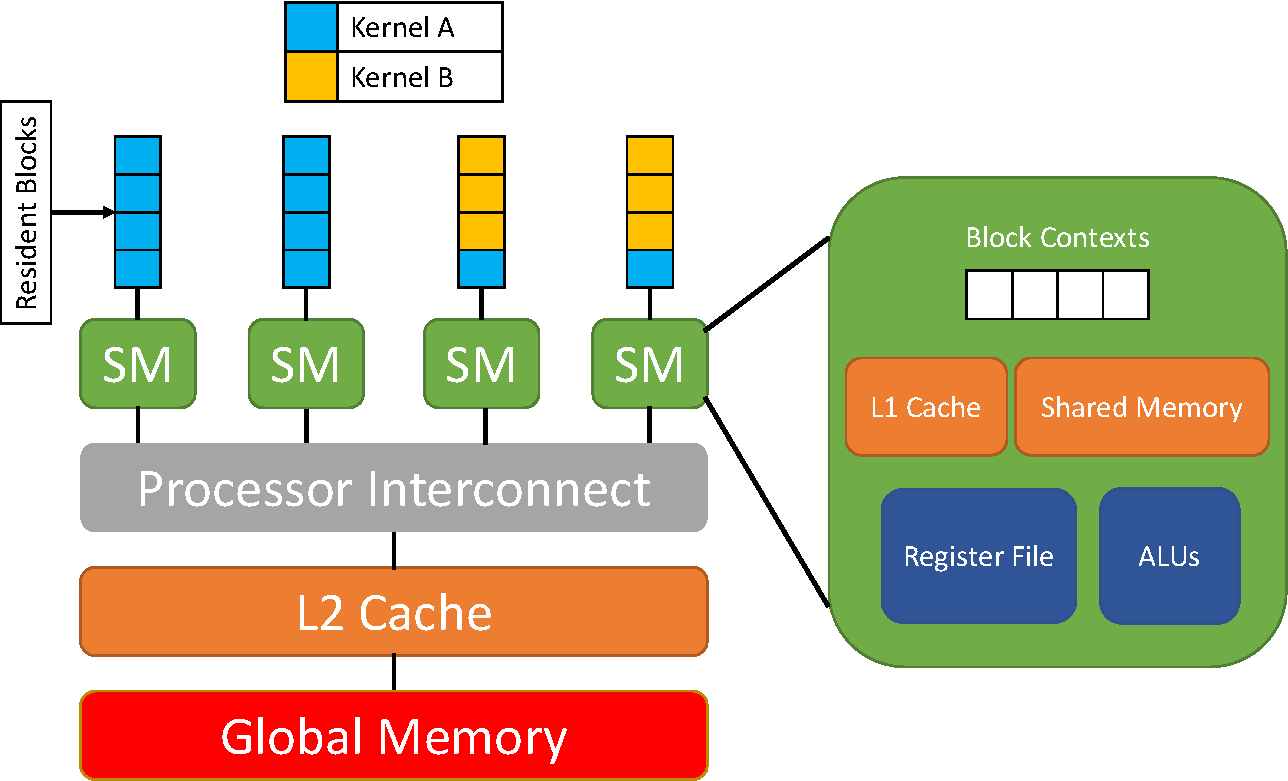
\includegraphics[width=\linewidth]{figures/gpu_diagram_cropped.pdf}
		\caption{Graphics Processing Unit (GPU)}
		\label{fig:gpu}
		\end{minipage}
	%    subfloat[fig:gpu]
		\hfill
		\begin{minipage}{0.45\linewidth}
		%\centering
		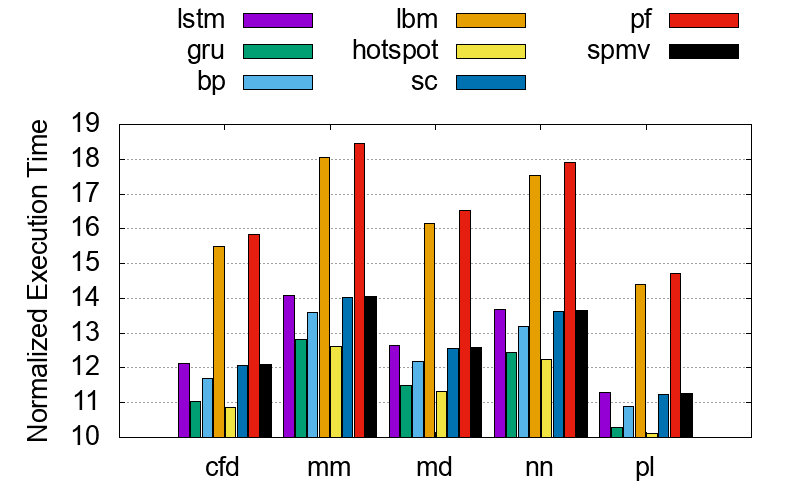
\includegraphics[width=\linewidth]{figures/seq_time.png}
		\caption{QoS violation for co-runs when the GPU is unpreemptable.}
		\label{fig:qos}
		%\vspace{-0.5cm}
		\end{minipage}
		\vspace{-0.6cm}
	\end{figure}

Conceptually, all the thread blocks of the launched kernels wait in a queue.  The hardware implements a FIFO thread block scheduler, which dispatches the waiting thread blocks to SMs as long as the available hardware resource can satisfy the resource demands. Hence, a kernel's thread blocks are guaranteed to be scheduled first before any other thread block of a later launched kernel.

Starting from the Fermi architecture, NVIDIA GPUs support concurrent kernel execution.  Later, NVIDIA introduced the Multi-Process Service (MPS), which enables kernels from  different applications to be executed simultaneously on the same GPU. However, due to significant context switch overhead,  the GPU hardware does not support temporal core sharing.  Consequently, the co-running kernels spatially share a GPU only  when the earlier launched kernel cannot consume all the computational resources. %This situation happens in the following two cases.  First, the earlier launched kernel only subscribes a small number of thread blocks. Second, the earlier launched kernel is about to finish its execution. As seen in Figure 1, the overall resource requirement of kernel A's remaining thread blocks  is so small that the greedy scheduler dispatches kernel B's thread blocks on the device such that kernel B's thread blocks will co-run with those of   kernel A on the last two SMs. 
Due to the organization of the hardware, Fig.~\ref{fig:gpu}  shows an interesting resource sharing scenario. The co-running thread blocks  from both kernel A and B on the same SM compete to use the L1 cache and ALUs and all the currently running thread blocks contend for use of the interconnect, L2 cache and global memory bandwidth.
%\subsection{QoS Issues in Co-Located GPU Applications}
%Most cloud service platforms nowadays employ GPUs \nadd{because of their high throughput and low cost}. But as pointed out by Chen  et al.~\cite{Chen+:ASPLOS16}, the GPUs may experience very low utilization  due to the diurnal pattern and the dynamic behaviors of GPU applications.  A natural solution similar to what exists in CPU-based platforms is \nsout{to co-locate  applications to share the same GPU}{multitasking where multiapplications share the hardware resources}. \nadd{There are two alternatives for multitasking on GPUs, spatial and temporal sharing.} While the co-location indeed improves \nadd{hardware} utilization,  uncoordinated co-running \nadd{applications may} introduce\nsout{s}{} severe performance interference \nadd{to others}and  \nadd{such interference will leads to} violat\nsout{es}{ion} \nadd{of} the QoS requirement of user-facing applications. 
%Baymax models the interference on data transfer between the CPU and the GPU  and the contention on GPU computational resources~\cite{Chen+:ASPLOS16}.  Based on a runtime system, it carefully manages data transfers and reschedules  kernel executions to mitigate the QoS violation issue. However, Baymax assumes  the GPU cannot be preempted, so once a kernel is launched,  it may monopolize the whole GPU for a long time, leading to unacceptable  performance degradation for the waiting kernels. In this paper, we  focus on the complicated problem of GPU core sharing between co-running  GPU applications and assume that the contention on data transfer is handled by the model proposed in Baymax.


\section{Motivation and Challenges}
\label{sec:motiv}
\vspace{-.2cm}	
	%\begin{figure}
	%	\centering
	%		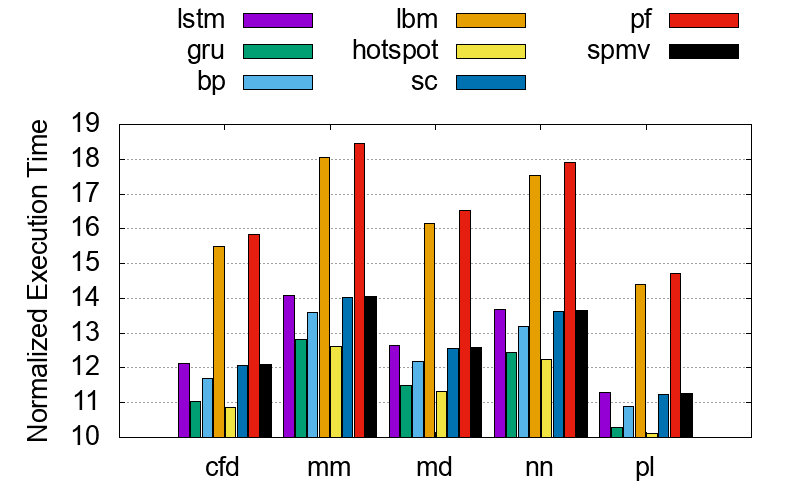
\includegraphics[width=8cm]{figures/seq_time.png}
	%	\caption{QoS violation for co-runs when the GPU is unpreemptable.}
	%	\label{fig:qos}
		%\vspace{-0.5cm}
	%\end{figure}
	
\subsection{QoS Issues of Non-Preemptable Kernels}
\label{sec:non-preemptable}
To understand the detrimental effect of non-preemptable kernel execution on QoS violation, we run 40 pairs of kernels (details in Section~\ref{sec:eval}) on an NVIDIA Volta GPU. Fig.~\ref{fig:qos} shows the performance degradation of the LC kernels when they are immediately launched after the BE kernels shown on the X axis.  Observe that QoS is violated for all the pairs even if the QoS target is as large as 10 times of the corresponding solo-run execution time when sharing is disabled. This is because the entire time the BE kernel is finishing normally, the LC kernel has to wait in queue, a clearly unacceptable solution.
%\nsout{Note that rescheduling kernels, 
%no matter how intelligent the algorithm is, cannot completely solve this problem.}{}
% 
%phenomena reflects the fact 
%It indicates that rescheduling strategy%, 
%no matter how intelligent the algorithm is, 
%cannot completely solve the problem of our concern.
%Since it is %\nsout{hard}{}
%already quite difficult, if not impossible, for us to predict the 
%arrival time of the LC kernels, launching a BE kernel without 
%any control on its resource usage may %\nsout{render 
%the whole GPU unusable for LC applications.}{}
%prevent LC applications from being executed because 
%all the resources have been claimed by the BE kernel. %According to the scheduling policy, LC applications 
%have to wait until the BE kernel is done. The QoS target is most likely violated in this case.
	
\subsection{Scalability Issues of Preemption-Based Solutions}
\begin{figure}
\vspace{-0.4in}
		\centering
		\begin{minipage}{0.45\linewidth}
		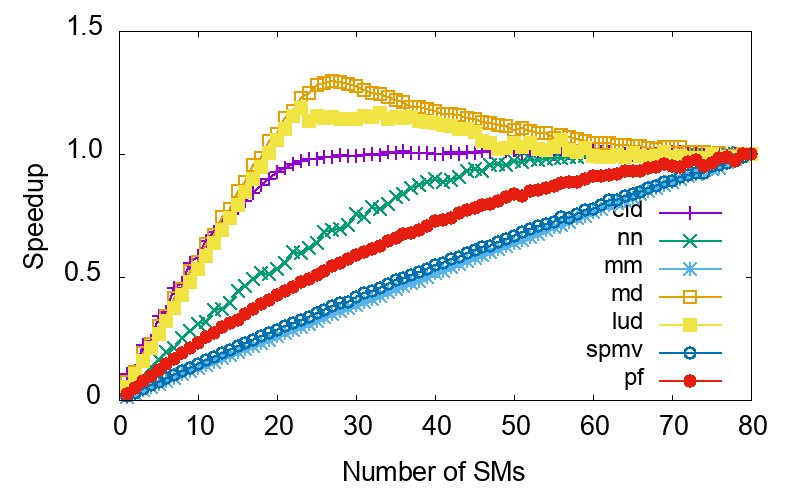
\includegraphics[width=\linewidth]{figures/solo_scalability/sm_scale_new.png}
		%\vspace{-0.2cm}
		\caption{Solo-run scalability with respect to the number of SMs}
		\label{fig:solo-sm}
		\vspace{-0.5cm}
	\end{minipage}
	\hfill
	\begin{minipage}{0.45\linewidth}
		\centering
		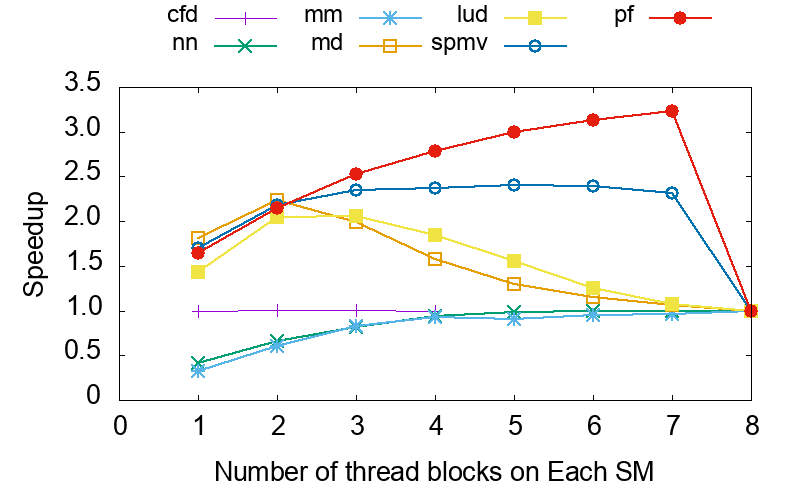
\includegraphics[width=\linewidth]{figures/solo_scalability/blk_scale_mul.png}
		%\vspace{-0.2cm}
		\caption{Solo-run scalability with respect to the number of thread blocks on each SM}
		\label{fig:solo-bl}
		\vspace{-0.5cm}
	\end{minipage}
	\end{figure}
	%\vspace{-0.8cm}
Recent work, such as FLEP~\cite{Wu:ASPLOS2017} and Effisha~\cite{Chen:PPoPP2017}, has proposed low-overhead software-based mechanisms to  realize preemption on GPUs.  With the capability of preemption, we can easily address the QoS issue by preempting  the BE kernel whenever an LC arrives. However, the drawback of preemption is that LC kernels monopolize all the available resources regardless of how efficiently it will utilize them. We show the scalability of 7 benchmarks in Fig. \ref{fig:solo-sm} and Fig.~\ref{fig:solo-bl} when we respectively increase the number of SMs and the number of thread blocks within each SM. Since the default scheduling uses up the SMs and thread blocks, the results show that less resource does not necessarily lead to worse performance. Moreover, different applications may have different scaling characteristics. For example, MM (matrix multiplication) prefers more computational resources, while MD's performance culminates with a small portion of the resources (i.e., 26 SMs or 2 thread blocks per SM).

% Figure \ref{fig:solo-sm} shows speedups of different applications with
% the number of SMs where there are 8 (4) TBs are scheduled on each SM and figure 
% \ref{fig:solo-bl} is scalabilities of the number of TBs on each SM. The size of 
% a TB is 256. Note all the kernels are able to run 8 TBs on an SM except CFD because each CFD thread uses 52 registers. 
%The idea of SM-centric transformation ~\cite{Wu+:ICS15} is adopted to show scalabilities of the kernels (details in Section~\ref{sec:system}).
%The benefit is that we have the ability of fine tuning the thread blocks being yielded to an LC kernel. We are able to
%control how many SMs to use and how many thread blocks to run on each used SM by an LC 
%application.
% These two figures tell us the following important things regarding to resource allocation.
%\begin{enumerate}
%\item 
% First, less resources could have positive speedup, that is, more resources don't guarantee better performance. %In Figure \ref{fig:solo-sm}, the performance of MD
%and LUD is linearly proportional to the amount of resources when the number of SM is less than 20. The speedup will be larger than 1 around 23 SMs and then the performance will start to decrease as 
%more resources are given to the applications. The same phenomena occurs in the scalabilities with respect to the number of TBs on each SM as well. 
%\item 
% Second, the performance could be saturated when partial resources are allocated. %This fact is reflected by the CFD and NN in Figure \ref{fig:solo-sm} 
% %and by NN and MM in Figure \ref{fig:solo-bl}. The CFD kernel's performance is saturated when 20 SMs are allocated, while NN saturates around 50 SMs. 
% %\item 
% Third, given the same amount resources, the performance of an application could have significant difference for different configurations. 
%       %Take the PF application as an example. Assume that
% %the application is given a half of the resources. The configuration (40, 8) will have speedup less than 1 while the configuration (80, 4) provides more than 2X speedup. 
% Our notation is that
% the first component of the configuration tuple is the number of SM being used and the second one is the TBs on those SMs.
% %\item 
% Fourth, the scalability is case dependent. %Obviously, it could be super-linear, linear and sub-linear based upon the observation on all 
% %the curves in two figures.
% %\item 
% Fifth, the hardware is generally underutilized. %An application could possibly oversubscribe resources if it runs alone on a GPU. The oversubscribing provides either 
      %no speedup or slowdown. The excessive resources could be freed up for better hardware utilization without hurting applications' performance. 
%\end{enumerate}
%}

	%\begin{figure*}
	%	\centering
	%	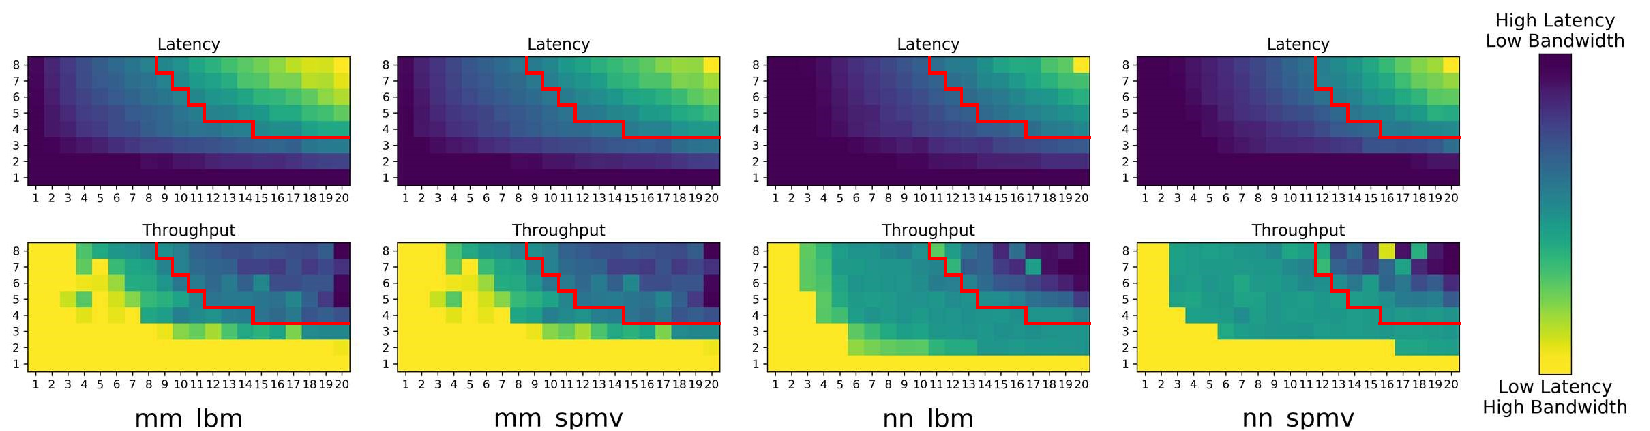
\includegraphics[width=\textwidth]{figures/corun_scalability_cropped.pdf}
	%	%\vspace{-0.5cm}
	%	\caption{Co-Run Scalability}
	%	\label{fig:corun-scalability}
	%	%\vspace{-0.15cm}
	%\end{figure*}
	\subsection{Spatial Co-Running and its Challenges}
%The rescheduling approach and the preemption-based approach are just two extreme points in a rich 
%design space of GPU spatial sharing among co-running applications. 
In order to run a pair of BE and LC application simultaneously, we need a mechanism for the BE application to be able to yield resources (entire SMs or thread block slots of SMs) to the LC application. Though the reduced resource availability and introduced contention cause slowdown for both kernels, we observe such a mechanism allows one to produce a better trade-off between QoS guarantees and overall GPU utilization. 
%We care about only the slowdown of the LC kernel and the overall throughput of the co-run pair.
%Therefore, 
% Such a mechanism allows one 
% to produce a better trade-off between QoS guarantees and overall GPU utilization. This leaves the following goals for this paper: \\
% %\begin{itemize}
% 	1. Better saturate GPU resources by spatially co-running two kernels rather than one.
% 	\\
% 	2. Keep the run time of the Latency Critical (LC) kernel under its QoS deadline \\
% 	3. Maximize the overall throughput of a BE-LC pair subject to latency constraint  %\end{itemize}
		%In order to combat poor resource utilization in GPUs, we suggest that a finer-grained sharing approach is required. Even when a whole GPU is occupied with thread blocks, it is not necessarily being maximally utilized, as suggested by the performance saturation shown in Figures \ref{fig:solo-sm} and \ref{fig:solo-bl}. Combating this is especially important at the datacenter scale where poor resource utilization drives up costs for GPU usage costs massively. Idle GPUs which only run QoS sensitive tasks and sit idle in between exacerbate this problem further. Running thread blocks from two kernels in a spatially-shared environment should make better use of some underutilized resources and make a more dynamic allocation methodology possible. This section will consider the differences between solo-run and co-run scalability to explore feasibility.
		%\par Unless a kernel manages to fully utilize on all shared resources simultaneously, there is potentially an opportunity to better utilize all the available hardware.
		%\par In order to combat poor resource utilization in GPUs, we can transform the BE application to yield resources for the co-running LC application. Consequently the kernels interfere with each other causing performance degradation. 
		
	\begin{figure*}%[h]
	\vspace{-0.5cm}
		\centering
		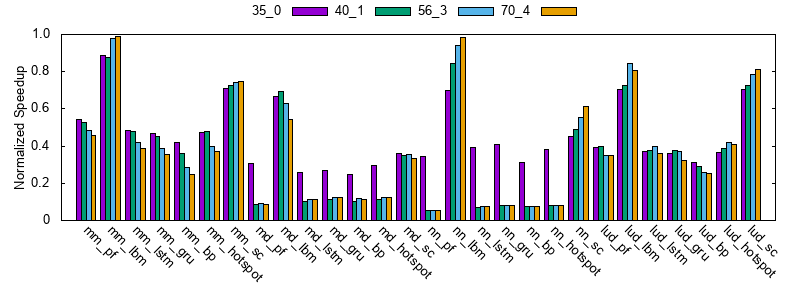
\includegraphics[width=\textwidth,height=3cm]{figures/mot_qperf.png}
		%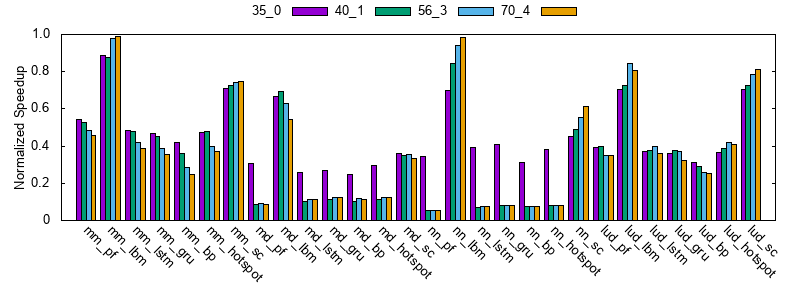
\includegraphics[width=9cm]{figures/mot_qperf.png}
		%\vspace{-0.2cm}
		\caption{LC kernel speedup with 280 thread blocks being allocated}
		\label{fig:corun_perf}
		\vspace{-0.5cm}
	\end{figure*}
To understand the complexity of the interference due to co-running, we run 40 kernel pairs with $280$ thread blocks allocated to each of the LC kernels. Fig. \ref{fig:corun_perf} shows the performance degradation of the LC kernels with four different configurations. On the X axis, the notation $A$\_$B$ represents a BE kernel $A$ co-running with a LC kernel $B$. Observe that the slowdown varies significantly across LC kernels or even the co-runs of the same LC kernel with different BE kernels. Fig.~\ref{fig:corun_thrpt} reports the overall throughput improvement (defined in Section~\ref{sec:eval}) and demonstrates the difficulty of predicting the best configuration for the co-runs.

% and \ref{fig:corun_thrpt}. 
% The notation used in the paper is the following. %The first component in the co-run pair is BE application, while the second is LC kernel. 
% The first number and the second one in SM configuration is the number of SM being yield to LC kernel and the number of TBs on these SMs, respectively. These two 
% figures shows that different pairs have different preference toward resource allocation. The resource allocation becomes even more complicated when the 
% QoS and throughput are taken into account. %For example at 5X QoS , the pair MM\_BP prefer inter-SM sharing from both QoS and throughput perspectives while the pair vote for the configuration 40\_1 and 
%NN\_LBM favors intra-SM 70\_4 sharing for both QoS and throughput. MM\_GRU likes intra-SM for throughput but inter-SM for QoS performance. Note that there is nothing special
%for $280$ TBs for LC kernel. %The same phenomena could be observed for difference total number of TBs. %The rule of thumb is that this number 
%should have as many as possible divisors between 1 and 8 to see such difference. 
%Therefore, 
% Different pair prefers different resource allocation to maximize
% the throughput even if the QoS is satisfied. %This is the focus of our paper.
%To understand the complexity of the interference due to spatial co-run\nsout{ning}{}, 
%we use MM and NN as BE applications and SPMV and LBM as LC applications, 
%and co-run each BE-LC application pair. For simplicity, we allow the BE application 
%to yield an arbitrary subset of SMs and the same number of thread blocks on each of those SMs. 
%Since the GPU has \nsout{20}{80} SMs and each SM can \nsout{run}{accommodate} up to 8 thread blocks due to the hardware limit, 
%each co-run pair has \nsout{160}{640} configurations for spatial sharing. Figure~\ref{fig:corun-scalability} 
%shows the performance degradation of the co-running applications. 
%In each column, the top figure shows the performance degradation for the LC application 
%and the bottom for the BE application. The top-right corner of each figure indicates 
%that the BE application yields the whole GPU to the LC application, maximizing QoS, 
%but providing no throughput to itself. Darker color means worse LC performance, 
%but higher BE throughput. The overall trend is clear and intuitive: 
%Yielding more resource improves the performance of the LC application but degrades the performance of the BE application.
\vspace{-0.7cm}
	\begin{figure*}[h]
		\centering
		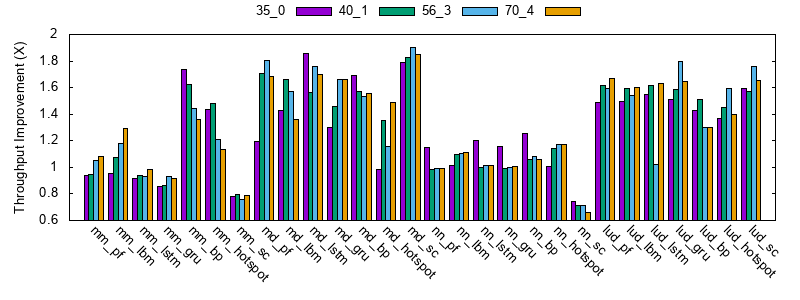
\includegraphics[width=\textwidth,height=3cm]{figures/mov_thrpt.png}
		%\includegraphics[width=9cm]{figures/mot_thrpt.png}
		%\vspace{-0.2cm}
		\caption{Overall throughput improvement}
		\label{fig:corun_thrpt}
		\vspace{-1.3cm}
	\end{figure*}
%From the boundary represented by the red curve to the top-right corner, 
%we have all the configurations that can satisfy the QoS requirement of the LC application. 
%Ideally, we should chose a configuration (very possibly on the boundary) in this region 
%which leads to minimum performance degradation for the BE application. 
%A naive online brute-force approach that tries all possible configurations and 
%chooses the optimal configuration would take too long and significantly violates QoS in the process.  
%For example, for the nn and spmv kernel co-run, 135 of the 160 runs violate QoS. 
%Unfortunately, the substantial differences between kernel behavior with and without 
%contention means the solo-run data is not very helpful for prediction. 
%The problem is especially challenging based on how different the degradation patterns 
%can be for different co-runs. For instance, co-runs involving the NN kernel experience
%much faster degradation of the QoS performance with fewer SMs than co-runs with MM. 
%Further, while a seemingly plausible solution is to profile all co-run configurations 
%offline to find the optimal configuration, it is not practical 
%because the applications may not be available offline, especially in a data center setting 
%where users may submit arbitrary applications. 
% In summary, to achieve the goals, this paper addresses the following challenges:
% %\begin{itemize}
% 	%\item 
%  estimating the co-running performance of kernels without extensive benchmarking,
% 	%\item 
% searching for the configuration whose throughput is maximized QoS is satisfied and %among many possible configurations for maximum throughput among those that satisfy QoS \\ %\item 
% 	minimizing the time taken to complete the configuration search
%\end{itemize}

\section{FLARE}
\label{sec:system}
\vspace{-.2cm}
% 	\par In this section we introduce FLARE, a system to enable flexible sharing 
%     of GPUs between LC and BE applications to improve hardware utilization. 
    %The purpose of spatial sharing among applications is to improve GPU resource utilization.
    %In addition, FLARE dynamically selects configurations to improve resource utilization. 
    %Furthermore, FLARE
    %dynamically explores the configuration space and 
    %searches for the best configuration, which satisfies the QoS requirement and in the meantime 
    %the overall co-run throughput of the pair is maximized.
	
	%\subsection{Goals}
	%	\par The primary design goal of FLARE is to maximize the overall throughput 
    %    of a co-run pair subject to QoS constraints on LC applications. 
    %    Datacenters often co-locate applications on shared servers to 
    %    improve resource utilization. But GPUs lack the fine-grained context switching 
    %    and preemption features of CPUs, making sharing them more difficult. 
    %    On shared GPUs, FLARE improves hardware utilization by safely sharing 
    %    the GPU between BE and LC applications.
%		\par FLARE is designed to consider the trade-offs between 
    %    latency and throughput caused by different co-run configurations. 
    %    The system must configure co-runs to maximize the available throughput 
    %    while respecting QoS requirements. This needs to be done quickly, 
    %    with as few QoS violations along the way as possible. 
    %    Resource allocation occurs at the kernel level, 
    %    so the dynamic reconfiguration can only happen between runs.
	
	\subsection{System Overview}
		The goal of FLARE is to enable flexible sharing between LC and BE applications 
        and optimize resource partitioning 
        to enforce QoS as well as maximize overall throughput 
        of co-run pairs. %FLARE implements spatial sharing through Hyper-Q technique.
        FLARE addresses the trade-off between latency and throughput 
        based on offline and online dynamic search algorithms to quickly figure out an optimized co-running configuration. The system, as shown in Fig.~\ref{fig:system}, consists of the following three components: \\%Kernel Transformation, Initial Configuration Selection, and Online Refinement.\\
		\textbf{\textit{Kernel Transformation}} FLARE transforms the BE application 
        to allow it to yield an arbitrary number of thread blocks on each SM. 
        Note that we assume there is no access to the kernels of LC applications 
        submitted by users, so FLARE does not transform the kernels of LC applications.\\
		 \textbf{\textit{Initial Configuration Selection}} To address the problem of unavailable LC applications for offline profiling, FLARE co-runs pairs of diverse microbenchmarks with many resource sharing configurations to characterize the performance degradation space. Based on the characterization, when the LC application arrives, FLARE only profiles its kernel invocation once to quickly model the performance degradation for both the LC and BE applications. FLARE then selects an initial configuration to spatially co-run the applications. \\
		\textbf{\textit{Online Refinement}} During the co-running, FLARE collects the performance degradation timing data as feedback to dynamically adapt the next configuration to use. By using the co-run degradation data of microbenchmarks, FLARE intelligently skips configurations and quickly reaches the optimal configuration to use for spatial co-running.
		%Each new kernel needs to be transformed to support spatial sharing and benchmarked for a single run with NVIDIA's Cuda profiler $nvprof$ before it is ready to run. The profiling results are used to characterize the expected behavior of the kernel when co-running to select an initial configuration, then an iterative process refines that configuration online. Each QoS kernel has a deadline $T_{dl}$ which is at least as long as the solo runtime $T_{solo}$. As long as that deadline is met, the configuration is satisfactory and the only other concern is how much throughput the configuration can achieve.
\subsection{Kernel Transformation:
				Enabling Spatial Sharing}


%\vspace{-0.8cm}
\begin{wrapfigure}{l}{0.5\textwidth}
		\centering
		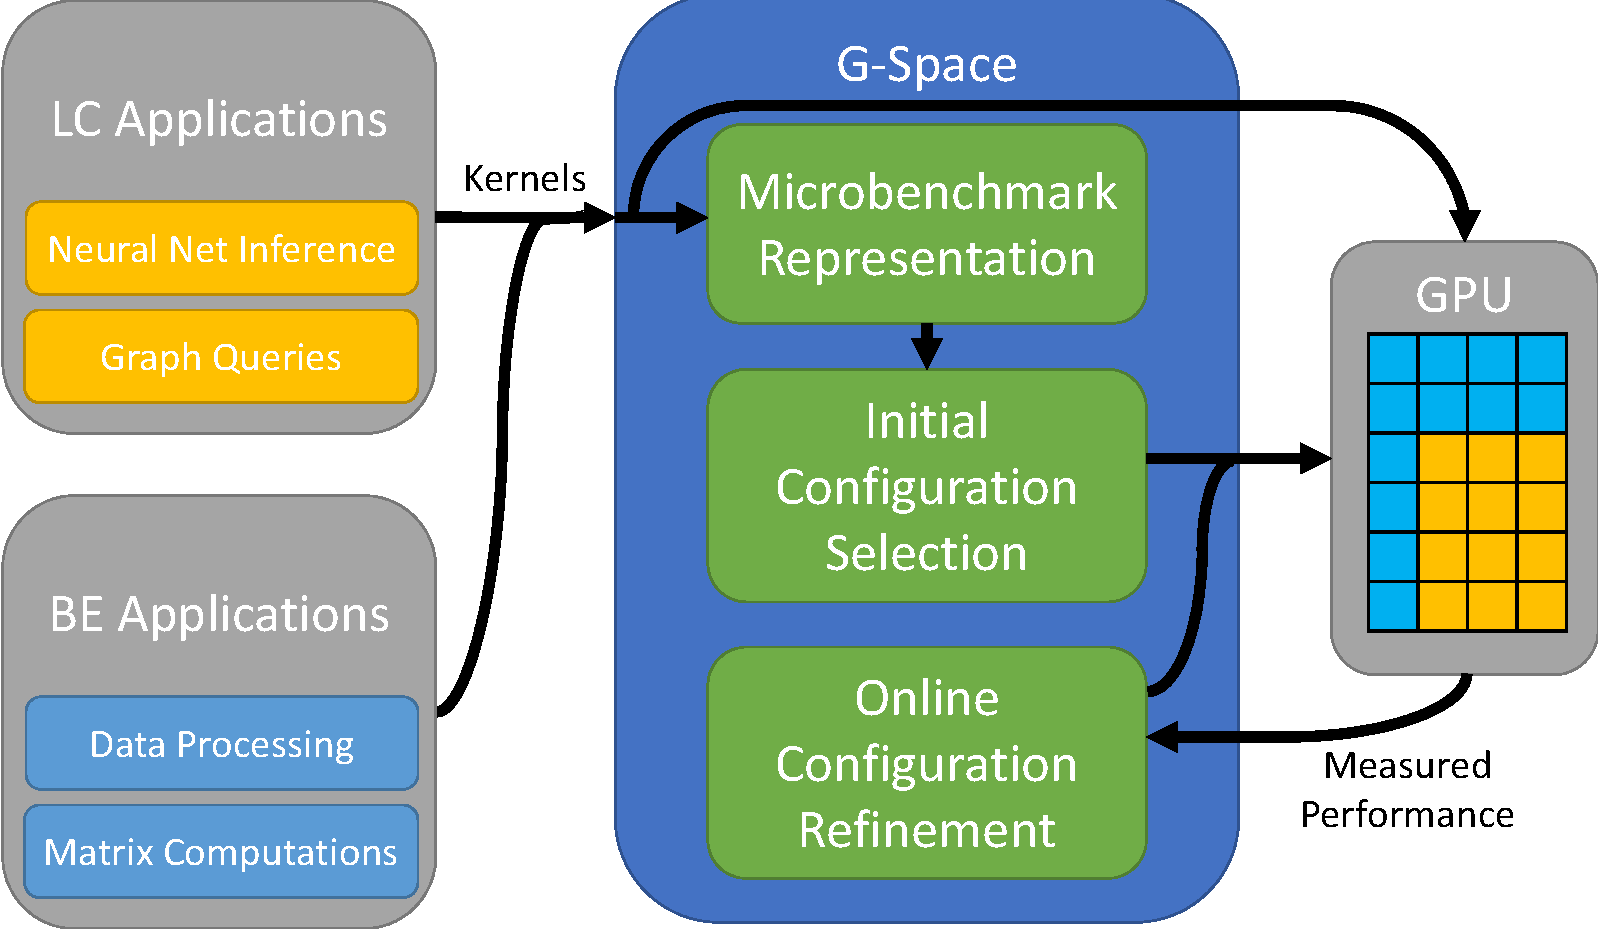
\includegraphics[width=\linewidth]{figures/system_diagram_cropped.pdf}
		\caption{The FLARE System}
		\label{fig:system}
		\vspace{-.2in}
		\end{wrapfigure}
		Kernel transformation enables the BE application to yield resources when a LC application is scheduled to the same GPU. The design, inspired by SM-centric transformation~\cite{Wu+:ICS15} and FLEP~\cite{Wu:ASPLOS2017}, runs just enough thread blocks to occupy the whole GPU. Specifically, given that a GPU has $N$ SMs and each SM runs up to $K$ thread blocks, FLARE schedules $N \times K$ thread blocks, each running the algorithm described in Fig.~\ref{fig:alg1}. Every thread block first invokes $get\_sm\_id()$ to obtain the ID of the host SM and then $atomic\_get\_blk\_id()$ to get its unique block ID on that SM, starting from 0. Each thread block stays in a while loop as long as there are tasks left to execute. At the beginning of each iteration, each thread block gets a unique ID. If a thread block ID is larger than the specified value $num\_blks[sm\_id]$, which is set by CPU, it means that the thread block needs to be yielded. To control the spinning overhead, we follow the approached proposed in~\cite{Wu:ASPLOS2017} to control the granularity of the tasks. Once the resource of the yielded thread blocks is released, the kernel of the LC application can acquire the resource and start co-running. After the LC application is finished, the BE application is notified and launches the same number of thread blocks as yielded to fully occupy the GPU again. 
		

		Although the algorithm enables arbitrary ways to yield thread blocks, it requires the CPU and GPU to share the array $num\_blks$, containing $num\_SMs$ elements, which may incur non-trivial communication overhead when $num\_SMs$ is large for high-end GPUs. To address this problem, FLARE uses the algorithm shown in Fig.~\ref{fig:alg2} to sacrifice flexibility for reduced overhead. In this new design, FLARE asks the BE kernel to yield the same number of thread blocks (i.e., $k$) on a subset of SMs (i.e., $n$). Since thread blocks of a kernel have similar behaviors and the SMs are homogeneous, we expect this simplified design to perform as well as the more flexible one.

		
		%The result of 
% 		This mechanism is summarized in the following workflow. 
%         %\begin{enumerate}
% 		%	\item 
% 			BE application claims all the resources on a GPU using exactly the same threads supported on the GPU;
% 		%	\item 
% 			When a LC application arrives, BE kernel yields resources;
% 		%	\item 
% 			The LC kernel greedily uses all yielded resources;
% 		%	\item 
% 			The BE application reclaims resources once LC kernel completes.
%			\begin{minipage}{0.48\linewidth}
%\begin{algorithm}[H]
%\caption{Arbitrary thread block yielding.}
%\tcp{Run by each thread block of BE kernel}
%\tcp{Global array num\_blks[num\_SMs]}
%\begin{algorithmic}
%\label{alg:alg1}
%\Function{BE\_Kernel}{$\cdots$} 
%  \State sm\_id = get\_sm\_id()\;
%  \State blk\_id = atomic\_get\_blk\_id()\;
%  \While{task\_queue is non-empty} {
%    \eIf{ blk\_id $>$ num\_blks[sm\_id]}{ quit\;
%    }{ 
%      \State task = pull\_task()\;
%      \State execute(task)\;
%    } 
%  } 
%\EndFunction
%\end{algorithmic}
%\end{algorithm}
%\end{minipage}
%\hfill
%\begin{minipage}{0.48\linewidth}
%\begin{algorithm}[H]
%\caption{Less exible thread block yielding to reduce overhead.} 
%\tcp{n: number of SMs to yield blocks}
%\tcp{k: number of blocks to yield}
%\begin{algorithmic}
%\label{alg:alg2}
%\Function{BE\_Kernel}{$\cdots$} 
%  \State sm\_id = get\_sm\_id()\;
%  \State blk\_id = atomic\_get\_blk\_id()\;
%  \While{task\_queue is non-empty} {
%    \eIf{ sm\_id $<$ n \textbf{and} blk\_id $>$ num\_blks[sm\_id]}{ quit\;
%    }{ 
%      \State task = pull\_task()\;
%      \State execute(task)\;
%    } 
%  } 
%  \EndFunction
%\end{algorithmic}
%cudaMalloc((void**)&num\_blks, sizeof(int)*num\_SMs)
%\end{algorithm}
%\end{minipage}
		%\end{enumerate}
		%\par By this mechanism, a particular number of blocks can be scheduled to each SM, so each kernel will have partial, simultaneous access to the GPU, enabling a spatial co-run. The allocations used by this paper will use a rectangular allocation of resources to the QoS kernel (k blocks on each of n SMs), and the rest of the GPU for the throughput kernel. Blocks running on the same SM will contend for that SM's computation resources and L1 cache space. All blocks on the GPU contend for the L2 cache space, main memory bandwidth, and PCIe bandwidth.
%\begin{wrapfigure}{l}{0.7\textwidth}
\begin{figure}
\vspace{-.2in}
\begin{center}
\begin{subfigure}[b]{0.3\textwidth}
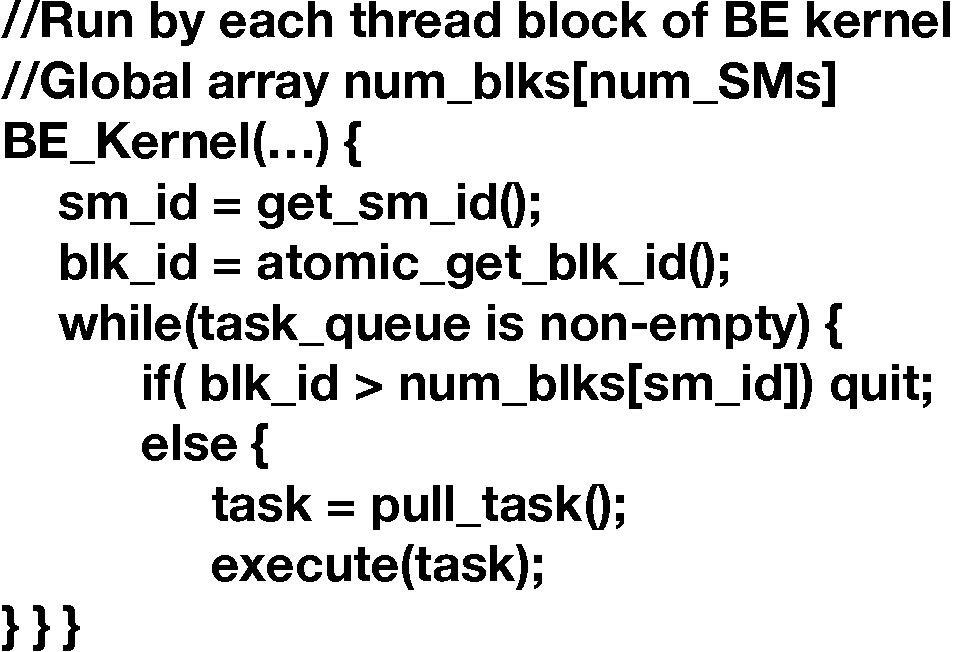
\includegraphics[width=\linewidth]{figures/trans_1-crop.pdf}
\caption{Arbitrary thread block yielding.}
\label{fig:alg1}
\end{subfigure}
\begin{subfigure}[b]{0.4\textwidth}
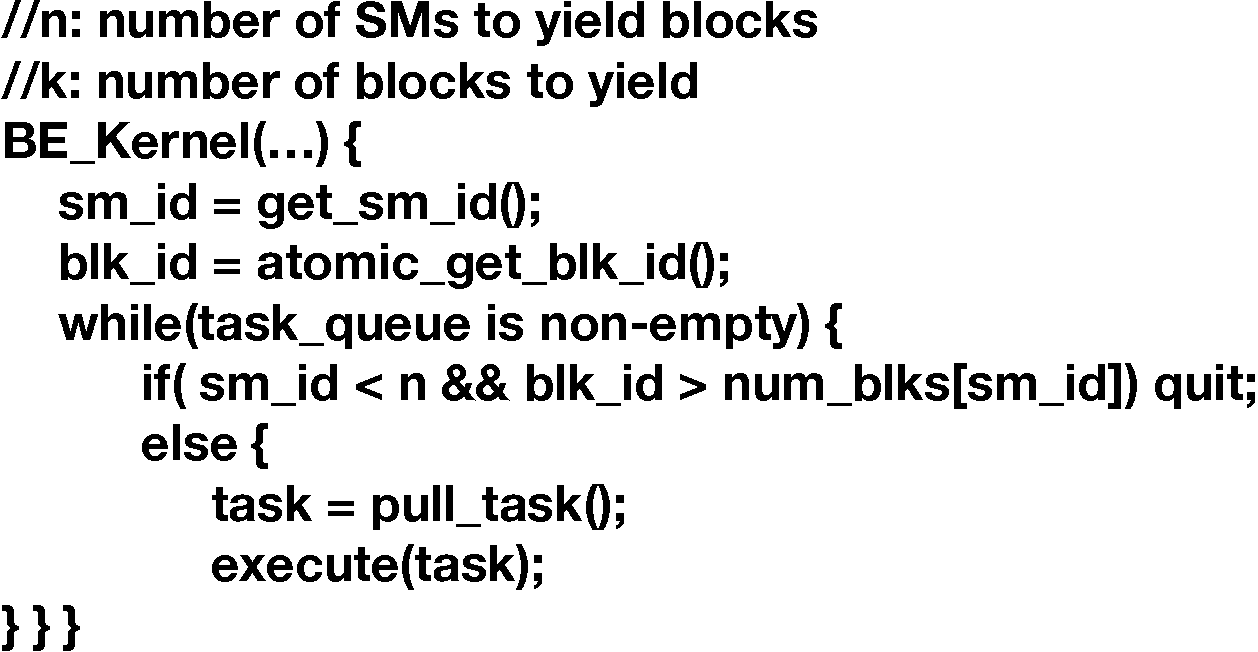
\includegraphics[width=\linewidth]{figures/trans_2-crop.pdf}
\caption{Less flexible thread block yielding to reduce overhead.}
\label{fig:alg2}
\end{subfigure}
\end{center}
\caption{Transformed BE kernels to allow spatial co-run.}
\vspace{-.5in}
\end{figure}
%\end{wrapfigure}
\subsection{Initial Configuration Selection:
				Microbenchmark Driven}
				\label{sec:initial}
		Due to the large spectrum of LC applications, FLARE cannot exhaustively profile BE-LC co-run pairs to find the optimal configuration. Instead, FLARE estimates the performance of BE-LC co-runs using microbenchmarks. Each kernel is matched with microbenchmark configurations that best represent its solo-run profiling statistics. Designing microbenchmarks  that represent real-world applications is not easy, because the performance of a kernel is affected by many factors and the importance of each factor varies for different kernels. But the relevant features should be those related to resources for which the kernels contend when co-running. Out of the 120 performance counters of NVIDIA's $nvprof$ profiler, we select the following 7 metrics which reflect or affect resource contention:
		%\begin{itemize}
		%	\item 
			L1, L2 cache hit rate,
		%	\item 
			DRAM, L2, and L1 bandwidth utilization,
		%	\item 
			arithmetic intensity, 
		%	\item 
			and total number of instructions. 
		%\end{itemize}
        
		To produce microbenchmark instances with varied features, we design a parameterized 
        kernel with two parts. The first part loads a 1-D array and the second part 
        contains a loop that performs pure arithmetic operations on the loaded data in each iteration. 
        %Note that it is quite difficult to decouple the parameters used in micro-benchmarks to simulate metrics related to $L1$ and $L2$ cache.
        %Hence, the 
        The microbenchmarks use the following 4 parameters to sample the configuration space: {\em stride length} to specify the distance between memory accesses from adjacent threads and hence control spatial locality of each thread block, {\em overlap ratio} to specifying the overlap between working sets of adjacent warps, {\em iterations} to control arithmetic intensity by specifying the number of iterations of the loop and {\em the number of threads} to run in total.
		
	    With 9 different stride lengths from 0 to 128 elements (L2 cache line size), 5 different overlap ratios ranging from 0 to 0.2, 
        iteration counts from 1 to 4, and a fixed number 160K of threads, 
        there are 180 different configurations of the microbenchmark. 
        We find that the range of these metrics covers most real world applications by tuning these parameters.
     
        %above, 
         %The range of L1 hit rate of microbenchmarks is $\left[4\%, 60\% \right]$ 
        %and L1 hit rate of real world application is from $0.22\%$ to $64\%$. This rate can be further increased if we tune up the overlap ratio. 
        %The current value is large enough for our experiments.
        %L1 hit rate of our microbenchmarks almost cover the range of real world application. 
        %It has been confirmed by the profiling data that the stride length affects 
        %the hit rates. 
         %We find that microbenchmark arithmetic intensity falls 
        %between $\left[50\%, 98\%\right]$. The minimum value of arithmetic intensity is $50\%$ where all the instructions in the kernel are memory operation. 
        %Although the theoretical maximum value is $100\%$, this kind of application is useless. 
        
        %Each %one of these 
        %Instance is run under $nvprof$ to 
        %characterize its performance according to the 7 parameters above. 
        Running all pairs of these microbenchmarks on all possible co-run configurations gives a large input dataset for training models 
        to get a sense of the patterns that arise. %We evaluate two low-latency techniques for utilizing this dataset to predict performance degradation of application kernels. \\
%\begin{algorithm}[!ht]
%\caption{Microbenchmark pseudocode}
%\begin{algorithmic}
%\label{alg:micro}
%\Function{microbench}{data, stride, overlap, arithmetic}
%\State get\_block\_id()\;
%\State get\_warp\_id()\;
%\State calculate\_warp\_offset()\;
%\State i = 0\;
%\While{i less than arithmetic}{
%  \State pure\_arithmetic\_operations\;
%  \State i++\;
%}
%\EndFunction
%\end{algorithmic}
%\end{algorithm}
		Given 180 different instances of the microbenchmark, we co-run each pair of them 
        in all possible ways to spatially share the GPU, resulting in a total of $640 \times 640 $ co-runs. 
        %Note that the total is not half of that, because we need to use each instance to represent a BE workload and a LC workload. 
        %Each co-run has two sets of characterization features for the two micro-benchmark instances, respectively, 
        %a co-run configuration for resource partitioning, and the corresponding performance degradation data. 
        Based on these results, FLARE has the following two methods to select the initial configuration. \\
%\vspace{.2cm}	
\textbf{\textit{Linear Regression}} %The linear regression method builds a
%pair of models to predict the performance degradation for each of the two co-running kernels.
%Linear model have the same set of features: 14 profiled features from the two co-running
The linear model has 16 features: 14 profile features from two
microbenchmark instances and the SM configuration (i.e., $n$ and $k$ in Fig.~\ref{fig:alg2}). 
%The model, therefore, concatenates the two 7-element
%feature vectors and 2-element configuration vector into a single 16-element
%vector. 
The linear regression maps that 16-element vector onto the
1-dimensional output space describing either estimated latency or throughput.
FLARE uses all the data from the offline co-runs as training data to build the
linear regression model. % (i.e., training the weights). %After deployment, 
 FLARE profiles 
one iteration of a solo-run of the BE kernel and the LC kernel (when it becomes available) to obtain the 14
characterization features and combine them with the other two features to get the feature vector of co-run applications. Then FLARE uses the linear regression models to
estimate the co-run performance degradation given each of the co-run
configurations, and finally selects the one that satisfies QoS and maximizes throughput.
Since the linear models are quite lightweight, the initial configuration-selection based on this method has a trivial overhead.\\
%\vspace{.2cm}
\begin{wrapfigure}{l}{0.5\textwidth}
			\centering
			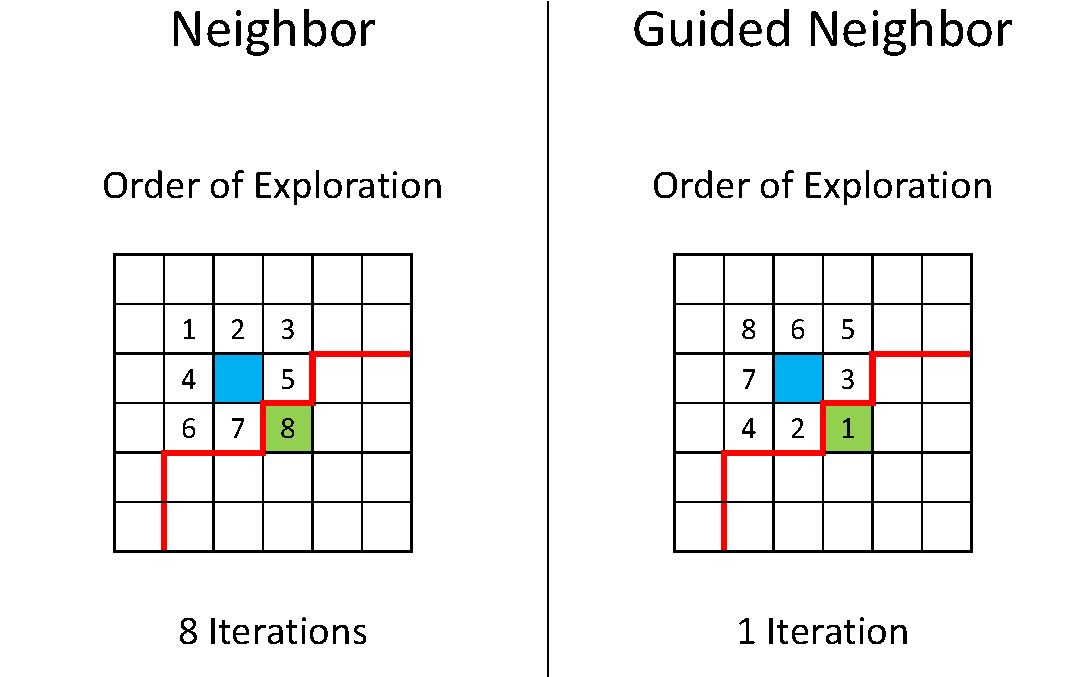
\includegraphics[width=\linewidth]{figures/new_search.pdf}
			\caption{Online search methods.}
			\label{fig:search}
			\vspace{-.3in}
			\end{wrapfigure}
		\textbf{\textit{Nearest Neighbor}} Like the linear regression method, the nearest neighbor method also profiles 
        one iteration of the BE and LC kernels to obtain their characterization features. For each kernel, 
        it then searches for a profiling characterization feature vector among the microbenchmarks that is the most similar 
        to that kernel in Euclidean distance. Specifically, each value of the 7-element feature vectors is normalized 
        to the range (0,1), and this method searches for the nearest microbenchmark feature vector $\vec{b}$ to the 
        feature vector of the real benchmark $\vec{m}$. 
        The nearest neighbor method selects the microbenchmark for which the quantity $\| \vec{m} - \vec{b} \|_2$ is minimized. 
        Each pair of representatives has offline-generated performance results on all of the co-run configurations available, 
        so this gives another estimate of the performance degradation across the configuration space. 
        Based on this, FLARE selects the configuration that satisfies QoS and maximizes throughput. This method requires no training and incurs negligible runtime overhead.
	\subsection{Online Refinement: Dynamic Reconfiguration}
%		\begin{figure}
%			\centering
%			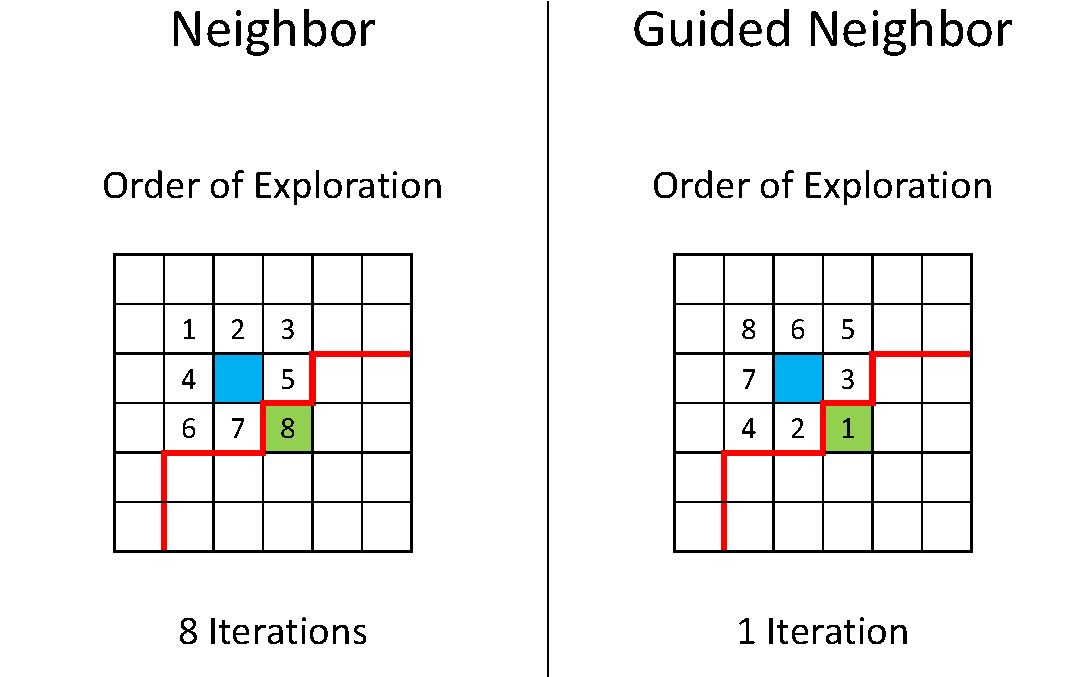
\includegraphics[width=8cm]{figures/new_search.pdf}
%			\caption{Online search methods.}
%			\label{fig:search}
			%\vspace{-0.8cm}
%		\end{figure}
The final configuration we select should be one with the highest possible throughput while still satisfying QoS. The initial configurations produced by the previously discussed methods are unlikely to match the globally optimal result every time. Therefore, configurations will need further refinement based on real performance feedback as shown in Fig. \ref{fig:system}. %In other words, FLARE needs to try a subset of configurations (i.e., execute the co-running kernels given those configurations) to figure out the optimal one. When FLARE tries a configuration, we say that configuration is explored. Note that due to the smooth performance degradation shown in Figure~\ref{fig:corun-scalability}, it may seem that a binary search-based approach can minimize the number of explored configurations. However, it does not directly translate to minimized search time. For example, exploring the extreme configuration of allocating most resources to the BE kernel may lead to unacceptable QoS violation for the LC kernel. So not only should these approaches find the optimal configuration, they should do it quickly and with as few QoS violations as possible. To achieve this goal, 
FLARE starts at the initial configuration and gradually explores the neighborhood to finally reach the optimal configuration. FLARE includes two approaches to performing the search as follows.\\
%\vspace{.2cm}
\textbf{\textit{Neighbor Search}} We demonstrate the idea of the first approach pictorially in Fig.~\ref{fig:search} (left panel). The cells represent configurations. Towards the bottom left corner, the configurations give more resources to the LC kernel. %Therefore, there should exist a continuous region of cells (included by the red line) that can satisfy the QoS requirement. 
The search process starts with an anchor cell (colored in blue), which should initially correspond to the configuration returned by the process described in Section~\ref{sec:initial}. It then explores all the 8 neighbor cells (the numbers show the order of the exploration), %which have not been tested before, 
and selects the best as the new anchor cell for the next round. Here the meaning of best is double-folded. When QoS is met, the best means that the overall throughput is optimal around neighbors. Otherwise, the best stands for the steepest decent of LC performance. This repeats until arriving at a cell where QoS is met and its throughput is the highest around its neighbors. \\
%The ``best'' neighbor configuration has different meanings when the anchor cell falls in the two different regions. In the regions of configuration that cannot satisfy the QoS, the best neighbor configuration is the one that minimizes the execution time of the LC kernel. Otherwise, the best neighbor configuration should minimize the execution time of the BE kernel. Therefore, when the initial configuration cannot satisfy the QoS, this approach tries to quickly enter the region that can satisfy the QoS and then maximize overall GPU utilization. This process works best on relatively low-noise data with a smooth performance degradation due to fewer allocated resources. It almost always eventually finds a configuration which satisfies QoS with better throughput than its neighbors, but may take many iterations to do so. To improve on this, it is important to maintain the same properties, but cut down on the total time taken. \\
%\vspace{.2cm}
\textbf{\textit{Guided Neighbor Search}} %With access to representative data from the micro-benchmarks, the patterns of the micro-benchmark and real kernel performance should be similar, even if not identical. This affords the opportunity to give some direction to the naive approach of the basic neighbor search. 
While the previous approach explores its neighborhood exhaustively, this approach searches first in the direction suggested by the microbenchmark data. Each neighbor cell has corresponding microbenchmark data, and therefore estimated QoS and throughput values associated with it. This gives some order to the neighbors in terms of their expected configuration performance, and we can simply explore the one with the best estimated performance. For example, Fig.~\ref{fig:search} (right panel) shows that according to the microbenchmark data, the bottom right neighbor configuration (labeled by 1) should produce the highest performance for the LC kernel. We then explore that configuration and select it as the anchor for the next round. By leveraging the microbenchmark data, we substantially decrease the number of steps required to converge. This process continues until it reaches a configuration where the QoS requirement of LC is satisfied and microbenchmark throughput is maximized. %, but have no guarantee of finding a higher quality configuration than the plain neighbor search, because the characterized performance degradation based on micro-benchmarks may not match that of the real applications. Hence, once the guided neighbor search terminates, we start a local refinement process to use the neighbor search process to improve QoS of the finally selected configuration.
%\vspace{.2cm}
%\textbf{\textit{Scalar Refinement Search}} The neighbor searches described above perform well when the initial configuration is close to the optimal configuration. Additionally, the guided search requires that the performance degradation pattern of the micro-benchmark exactly matches that of the application kernels. While we observe that the patterns are similar, the rate of degradation can differ significantly from the true pattern. We propose a hypothesis: that the micro-benchmark and application kernel performance degradation differences are equivalent to a multiplicative scalar difference in the QoS target. The red lines in Figure \ref{fig:corun-scalability} which separate configurations satisfying QoS from those that don't has an equivalent in the micro-benchmark space. The corresponding line in micro-benchmark space is typically substantially offset from the line that appears in that figure. For example, in the mm and lbm co-run there are 48 configurations which satisfy QoS with a QoS ratio of 2.0 (i.e., the QoS target is twice its solo execution time). Their representative micro-benchmark pair has 134 configurations which satisfy QoS for the same ratio, so the line is substantially offset toward the bottom-left. A similar line could be found by decreasing the QoS ratio used for the micro-benchmark. Scalar Refinement method can automatically perform this correction for the offset in an online fashion.
%This approach also starts at the configuration that was optimal for the micro-benchmark. Based on the performance data for that single run, we can adjust the micro-benchmark QoS ratio to better fit that result. If the result fails to satisfy QoS, the ratio needs to decrease to make it more restrictive as shown in Figure \ref{fig:search} (right panel). If it satisfies QoS by a wide margin, the ratio should increase to allow for a more aggressive configuration. Recomputing the micro-benchmark optimal configuration may give a new configuration, which we explore in the next iteration. This continues until the new and old configurations match, which happens very quickly. Figure \ref{fig:search} illustrates this process in terms of the line adjustment it implies. More precisely, scalar refinement adjusts the scalar $\gamma$ on the target QoS ratio $q$ for the micro-benchmark, such that the micro-benchmark search looks for configurations that satisfy a QoS ratio of $q \times \gamma$, with $\gamma$ initially 1. In subsequent iterations, if the real performance result exceeds the QoS target by a factor of $c$, then for the next iteration $\gamma$ will be decreased by an amount proportional to $c$. Conversely if the result over-achieves the QoS target by a factor of $c$, then $\gamma$ will be increased proportionally to $c$. The scalar $\gamma$, therefore, represents the increased or decreased restrictiveness of the QoS target assumed for the micro-benchmark to allow it to closely match the real boundary. We determine the proportional adjustments empirically to smooth the adjustment of $\gamma$ and maintain a small number of steps to convergence. While this method is not guaranteed to reach a configuration which satisfies QoS, it should be very close to configurations that do, and will likely have found a border configuration. So we also add a local refinement process the same as in guided neighbor search to enforce QoS of the selected configuration.
%\begin{minipage}{0.5\linewidth}
%\begin{algorithm}[!ht]
%\caption{Microbenchmark pseudocode}
%\begin{algorithmic}
%\label{alg:micro}
%\Function{microbench}{data, stride, overlap, arithmetic}
%\State get\_block\_id()\;
%\State get\_warp\_id()\;
%\State calculate\_warp\_offset()\;
%\State i = 0\;
%\While{i less than arithmetic}{
%  \State pure\_arithmetic\_operations\;
%  \State i++\;
%}
%\EndFunction
%
%\end{algorithmic}
%\end{algorithm}
%\end{minipage}
%\hfill
%\begin{minipage}{0.5\linewidth}
%\caption{Benchmarks}
%    \begin{tabular}{ | l | c | c | c |}
%        \hline
%        {\bf App.} & {\bf Source} & {\bf Description} & {\bf Role} \\ \hline \hline
%        CFD & Rodinia & finite volume solver & BE \\ \hline
%        MD  & SHOC & molecular dynamics & BE \\ \hline
%        MM & CUDA SDK & dense matrix multiplication & BE\\ \hline
%        NN  & Rodinia & nearest neighbor & BE \\ \hline
%        %PL & Rodinia & bayesian framework & BE \\ \hline
%        BP & Rodinia & backpropagation& LC \\ \hline
%        LBM & Rodinia & fluid dynamics & LC\\ \hline
%        HOTSPOT & Rodinia & thermo dynamics & LC \\ \hline
%        PF  & Rodinia & dynamic programming & LC \\ \hline
%        SC  & Rodinia & data mining & LC \\ \hline
%        SPMV & SHOC & sparse matrix multiplication & LC\\ \hline
%        TC  & \cite{text} & text classification & LC \\ \hline
%        CN  & \cite{Sutskever:ICML11} & text generation & LC \\
%        %CC  & \cite{Han:PACT2017} & connected component & LC \\
%        \hline
        %\hline
%    \end{tabular}
%    \label{tbl:apps}
%\end{minipage}

\section{Evaluation}
\label{sec:eval}
\vspace{-0.2cm}
%		\par Figure showing nvprof metrics for all 10 application kernels and the closest match from the microbenchmark. Figure showing similarity of microbench and kernel corun 2D spaces for one kernel pair. Use these figures to argue that we have a good way to get pre-generated data which mirrors the contention properties of the application kernels.
%		\par Show that the 2D spaces are off by nearly a constant in the QoS ratio, possibly another figure to show how close a constant factor adjustment gets them to matching

%\begin{figure}
%	\centering
%	\caption{Co-Running Windows Explainer}
%	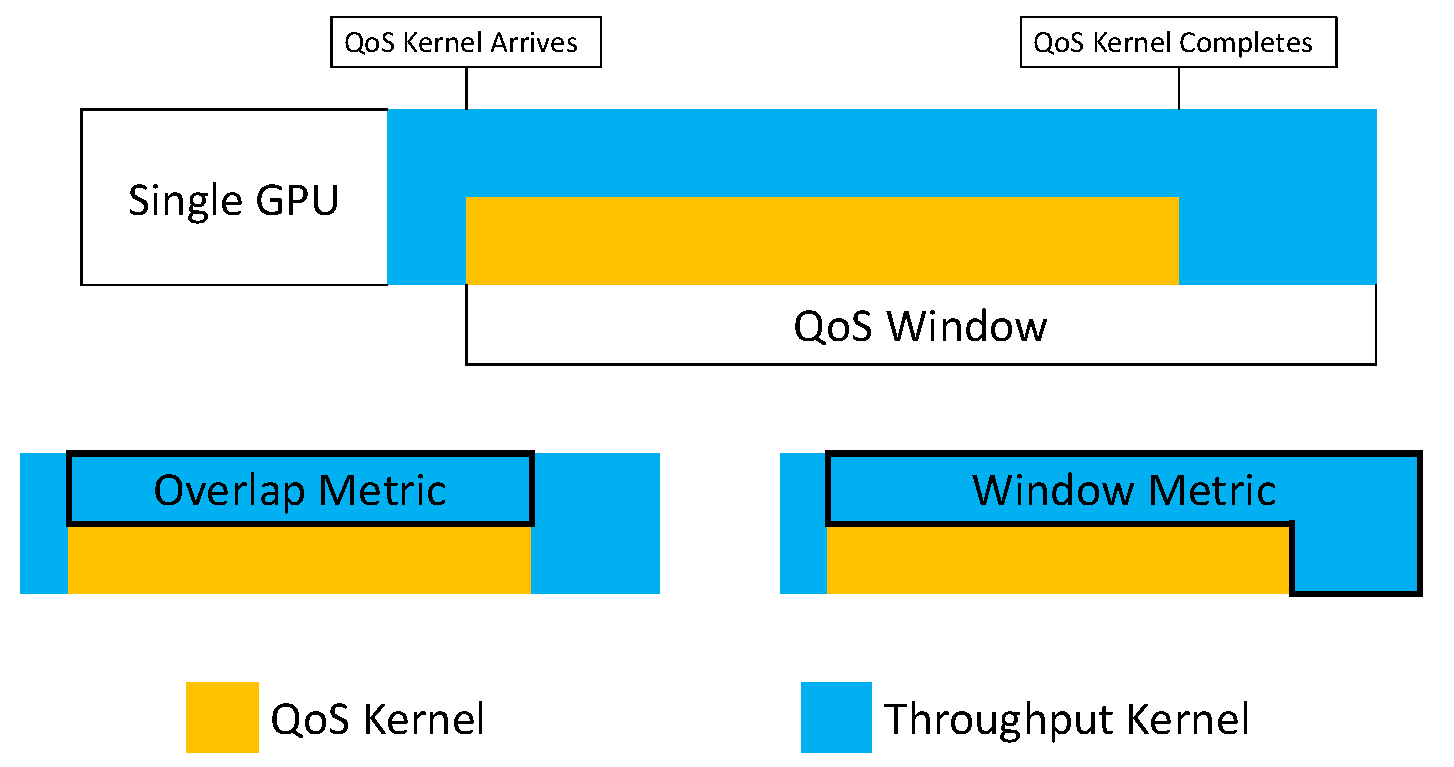
\includegraphics[width=8cm]{figures/corun_windows_cropped.pdf}
%	%\vspace{-1cm}
%	\label{fig:corun-windows}
%\end{figure}

%Short summary of this section
%\par This section presents the experimental results for the performance of the approaches presented in this paper.

\subsection{Experimental Setup}
\begin{figure*}
        \vspace{-1cm}
        \centering
        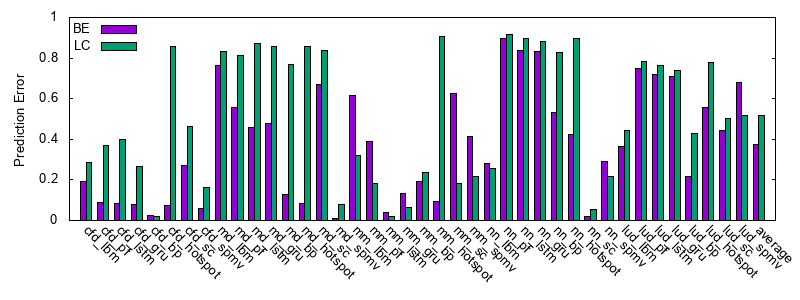
\includegraphics[width=\textwidth,height=2.5cm]{figures/new_error_res.png}
        %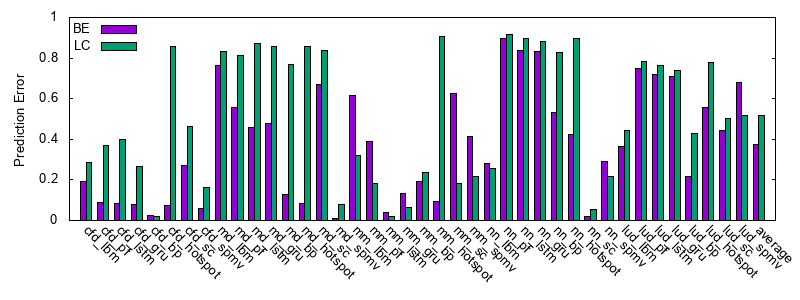
\includegraphics[width=\textwidth]{figures/new_error_res.png}
        \caption{Performance estimation error evaluation.}
        \label{fig:error}
        \vspace{-.5cm}
\end{figure*}
%\begin{table}
%\scriptsize
%\vspace{-0.5cm}
%\centering
%    \caption{System Setup}
%    \begin{tabular}{ c | c }
%        \hline
%        CPU & 2S Intel Xeon E7-4830 v3 @ 2.1 GHz \\
%        GPU & NVIDIA TITAN V100 w/ 12GB GDDR5X \\
%        \hline
%        OS & Ubuntu 16.04 x64 with kernel 4.4.0-128 \\
%        CUDA & Driver 418.56 CUDA SDK 10.1 \\
%        \hline
%    \end{tabular}
%    \label{tbl:system}
    %\vspace{-.5cm}
%\end{table}
\par We evaluate FLARE using an NVIDIA TITAN V GPU with 12GB onboard memory hosted by a server with an Intel Xeon E3-1286 v3 CPU and 32GB main memory. The system runs Ubuntu 16.04 with kernel version 4.4.0-141, NVIDIA driver 410.48, and CUDA 10.0.
%The table \ref{tbl:apps} shows
We focus our evaluation on eleven benchmarks and two real-world applications. The benchmarks are from three popular benchmark suites: Rodinia~\cite{Rodinia}, SHOC~\cite{SHOC},
and NVIDIA's CUDA SDK. Two real applications,
TC~\cite{text} and CN~\cite{Sutskever:ICML11}, represent deep learning inference workloads. TC uses an LSTM~\cite{LSTM} model to classify documents and 
CN uses a GRU~\cite{GRU} model to predict the likely next character given an input string. Both of these inference applications heavily utilize the GPU, and are classified as LC applications. We also evaluate SPMV (SHOC), SC, PF, HOTSPOT, LBM and BP (Rodinia) as LC applications and MD (SHOC), MM (CUDA SDK), NN, LUD and CFD (Rodinia) as BE applications. Only the BE applications require adaptation to yield resources, while the LC applications can run unmodified.
%The table also identifies which applications are classified as BE and LC applications
%shown by the ``Role'' column. Every co-run pair presented in this section is composed of one BE application and one LC application.
%The goal is to maximize the throughput achieved while still completing the QoS kernel within a deadline. Unless otherwise noted, that deadline is assumed to be 2 times the duration the kernel takes when running alone on the GPU, also referred to as a QoS ratio of 2.
%\begin{table}[ht]
%\centering
%\scriptsize
%\begin{minipage}
%\centering
%    \caption{Benchmarks}
%    \begin{tabular}{ | l | c | c | c |}
%        \hline
%        {\bf App.} & {\bf Source} & {\bf Description} & {\bf Role} \\ \hline \hline
%        CFD & Rodinia & finite volume solver & BE \\ \hline
%        MD  & SHOC & molecular dynamics & BE \\ \hline
%        MM & CUDA SDK & dense matrix multiplication & BE\\ \hline
%        NN  & Rodinia & nearest neighbor & BE \\ \hline
%        %PL & Rodinia & bayesian framework & BE \\ \hline
%        BP & Rodinia & backpropagation& LC \\ \hline
%        LBM & Rodinia & fluid dynamics & LC\\ \hline
%        HOTSPOT & Rodinia & thermo dynamics & LC \\ \hline
%        PF  & Rodinia & dynamic programming & LC \\ \hline
%        SC  & Rodinia & data mining & LC \\ \hline
%        SPMV & SHOC & sparse matrix multiplication & LC\\ \hline
%        TC  & \cite{text} & text classification & LC \\ \hline
%        CN  & \cite{Sutskever:ICML11} & text generation & LC \\
%        %CC  & \cite{Han:PACT2017} & connected component & LC \\
%        \hline
        %\hline
%    \end{tabular}
%    \label{tbl:apps}
 %   \end{minipage}
%    \vspace{-0.8cm}
%\end{table}
%\subsection{Compared Approaches}
%Section~\ref{sec:non-preemptable} shows that rescheduling-based methods may seriously
%violate QoS when the BE application has non-trivial workloads.
%Thus, we compare FLARE with preemption-based approaches proposed in EffiSha~\cite{Chen:PPoPP2017} and
%FLEP~\cite{Wu:ASPLOS2017}. Since these two approaches are similar, we only use FLEP as our baseline.\\
%FLARE proposes three ways to choose co-run resource partition configurations: model based, online search based,
%and hybrid. The model-based approach incurs trivial runtime overhead but may choose a poor
%configuration where a QoS target could possibly ruined, while the online search based approach may need to explor many configurations
%to find a desirable one.
%FLARE supports both linear regression and nearest neighbor
%methods for model-based configuration selection. Both model based approaches have flaws.
%See section \ref{sec:system} for why model based approach does not provide a better solution.
%Two scalability figures in section~\ref{sec:motiv} show that the relationship between resources and performance is quite compilicated.
%It is pointed out in section \ref{sec:motiv} that the performance of an application may not be linear in term of allocated resource. The relationship is quite complicated. And the nearest search
%implicitly assumes that configuration space is flat and each dimension in the configuration space has equal weight. In reality, the configuration space
%is a non-trivial topological space.
%Due to space limitations, 
%We evaluate the
%prediction accuracy of both methods but only use the nearest neighbor method in the
%model-based approach since the nearest neighbor method is much better than linear regression. A hybrid approach uses the model-based approach to select an initial
%configuration followed by a online search based approach to refine the configuration, which
%has the potential to perform the best among all the three approaches. Since FLARE supports
%two online search methods regardless of the initial configuration, namely neighbor search
%(NS) and guided neighbor search (GNS), we have
%2 hybrid approaches: NN\_NS and NN\_GNS, where the nearest neighbor method
%selects the initial configuration and based on this initial guess the following dynamic search methods refine the
%configuration. Therefore, in total we evaluate 5
%approaches included in FLARE: NN, NS, GNS, NN\_NS and NN\_GNS. To evaluate NS and GNS, we allocate a quarter of the GPU to the LC applications as the
%initial configuration. %\vspace{-0.3cm}
\subsection{Evaluation Strategy}
    We evaluate the performance of our approaches under the following scenario. %\begin{itemize}
		%\item 
		The BE application runs continuously and consumes the entire GPU when no LC application is present.
		%\item 
		When a LC application arrives, the BE application yields part or all of the computation resources on the GPU to the LC application and two applications start to run simultaneously on the device. %to run depending on the evaluated approach.
		%\item 
		The LC application has a QoS deadline, and if its execution time exceeds this deadline the QoS is violated.
		%\item 
		As soon as the LC kernel completes, the BE kernel reclaims all of the hardware resources and resumes running exclusively.
	%\end{itemize} 
    For this scenario, we always launch the BE kernel first and then start the LC kernel in a different CUDA stream. In order to compare with CUDA Multi-Process Service (MPS), we observe that simple SM-based partitioning gives the same performance results as MPS, and consider it as a possible configuration. Note that unlike FLARE, MPS does not support dynamic resource allocation. Once the application is launched, its allocation of the GPU resource cannot be changed. Thus, the MPS results in this section represent the best possible results MPS can produce.
    
    In this paper, throughput refers to the number of instructions executed per microsecond. We define the overall throughput of a co-run pair as,
    \begin{equation}
    P^c=\left(\text{INS}_{LC} +\text{INS}_{BE}^c\right)/T_{LC}^c
      %P_{A}^c = (T_{LC}^c - T_{LC}^s)/T_{LC}^c\times P_{BE}^s
    \end{equation}
    where $P^{c}$ is the overall throughput of co-run, $\text{INS}_{LC}$ and $\text{INS}_{BE}^c$ are the number of instructions of LC and BE applications during co-run, and $T_{LC}^{c}$ is the performance of a co-run LC kernel. %The throughput improvement%$T_{LC}^c$.
    We are going to compare this overall throughput with the sequential throughput during $T_{LC}^c$. 
    When a LC kernel arrives, the BE application will yield the GPU to the LC. Then the LC kernel starts to run and will be finished in $T_{LC}^s$. The BE resumes thereafter. But we only need to consider the number of BE instructions, $\text{INS}_{BE}^{tw}$, finished in time window $T_{LC}^c - T_{LC}^s$, because our interest is to see throughput improvement of co-run. Therefore, the sequential throughput is given by
    \begin{equation}
        P^s = \left(\text{INS}_{LC}+\text{INS}_{BE}^{tw}\right)/T_{LC}^c
    \end{equation}
    The ratio of $P^c$ to the sequential throughput $P^s$ gives us the throughput improvement.
    %Section~\ref{sec:non-preemptable} shows that rescheduling-based methods may seriously
%violate QoS when the BE application has non-trivial workloads.
%Thus, 

We compare FLARE with the preemption-based approaches proposed in EffiSha~\cite{Chen:PPoPP2017} and
FLEP~\cite{Wu:ASPLOS2017}. Since the two approaches are similar, we only use FLEP as the baseline.
FLARE proposes three ways to choose resource partitioning configurations: model-based, online search-based,
and hybrid. The model-based approach incurs trivial runtime overhead but may choose a poor
configuration where a QoS target could possibly be missed, while the online search-based approach may need to explore many configurations
to find a desirable one. This evaluation will demonstrate that the flaws in these approaches prevent them from achieving the best performance.
%Two scalability figures in section~\ref{sec:motiv} show that the relationship between resources and performance is quite compilicated.
Section \ref{sec:motiv} notes that the performance of an application may not be linear in terms of allocated resource. Worse, the resource contention due to co-running makes it even more difficult to statically predict the optimal configuration.
Since \textbf{NN} outperforms \textbf{Linear Regression} in all cases, we only show the results on the former.
A hybrid approach uses the model-based approach to select an initial
configuration followed by a online search approach to refine the configuration. %, which
%has the potential to perform the best among all the three approaches. %Since 
FLARE supports
two online search methods regardless of the initial configuration, namely neighbor search
(\textbf{NS}) and guided neighbor search (\textbf{GNS}).
It leads to two hybrid approaches: \textbf{NN}\_\textbf{NS} and \textbf{NN}\_\textbf{GNS}. %, where the nearest neighbor method
%selects the initial configuration and based on this initial guess the following dynamic search methods refine the
%configuration. 
Therefore, we evaluate 5
approaches included in FLARE: \textbf{NN}, \textbf{NS}, \textbf{GNS}, \textbf{NN}\_\textbf{NS} and \textbf{NN}\_\textbf{GNS}. %To evaluate NS and GNS, we select (40\_4) as the
%initial configuration.
%	\par To understand why, consider the following situation: \begin{itemize}
%		\item A LC kernel takes $T_{LC}$ time when running solo and has a QoS deadline of $T_{QoS} = 2 \times T_{LC}$ time.
%		\item The background BE kernel has performance $P_{BE}$ when running solo.
%	\end{itemize} 
%	
%And two possible configurations: 
%\begin{enumerate}
%		\item \label{config:full} The kernels co-run for the entire $T_{QoS}$ window, and the BE throughput while co-running is $\frac{3}{5} \times P_{BE}$. Because the kernels co-run for the entire window, that is also the average throughput for the window
%		\item \label{config:part} The kernels co-run for three-fourths of the QoS window ($1.5 \times T_{LC}$), and the BE throughput while co-running is $\frac{1}{2} \times P_{BE}$. After termination of the LC kernel, the BE kernel reclaims the whole GPU and runs for the remaining $T_{LC}$ time. This implies an average throughput of $\frac{5}{8} \times P_{BE}$ for the window
%	\end{enumerate} While configuration \ref{config:full} has the higher co-running BE throughput, the average for the entire window is lower than that of configuration \ref{config:part}. As long as the GPU gets at most 1 LC task to run per $T_{QoS}$ time, the average metric maximizes the overall throughput while satisfying QoS for incoming tasks.
%	\par The essential observation for the metric choice is that the opportunity cost of running a particular configuration in terms of lost throughput is all that matters as long as the QoS deadline is met. In most cases we observe the co-running configuration having lower opportunity cost than FLEP (which has an average throughput of $\frac{1}{2} \times P_{BE}$ for this situation), but this metric still helps select among possible configurations even if they all beat the FLEP configuration. We therefore use the average window throughput metric to evaluate our approaches in the remainder of this paper. The presented results are labeled according to the form <BE app>\_<LC app>.-0.3cm}
\subsection{Results}%{ on Benchmarks}
Due to limited space, we only show the results for 1.5X QoS, that is, the co-run latency of a LC kernel cannot exceed 1.5X its solo-run time. Fig.%~\ref{fig:throughput-results} and
~\ref{fig:throughput-results} shows throughput improvement %of the final selected co-run configuration of a pair
of FLARE with the best performing approach, \textbf{NN}\_\textbf{GNS}, and binary search-based SM allocation with MPS. %approaches in section \ref{sec:system} and binary search normalized to the throughput of %running the pair sequentially. % with QoS target equal to 1.2X of LC solo-run execution time.%and 
%1.5X QoS. %of LC solo-run execution time. 
%Since dynamic searches produces the same throughput improvement for the fin, we only plot
%the results obtained from \textbf{NN}\_\textbf{GNS} in the Fig. \ref{fig:throughput-results}. The difference is that the overhead of each approach differs.
%The selected configuration of %all the approaches 
%dynamic searches satisfies the QoS requirement
%after dynamic searches, while 
%NN %prediction %relies purely on the prediction and chooses configurations
%that 
%only achieves 37.6\% %and 58.2\% 
%of the global optimal throughput % for QoS target 1.2X and
%1.5X of LC applications' solo-run time 
%on average. By leveraging online search, all the other approaches perform
%significantly better than \textbf{NN}. %-only method. 
Observe that FLARE increases the average %overall 
throughput improvement by 38.8\% compared with FLEP. %and 139\% 
FLEP %, as well as other preemption-based approaches,
runs the LC application first to guarantee QoS and
then the BE application after the LC application, thus missing co-running opportunities to improve throughput.
%Fig. \ref{fig:throughput-results} %and \ref{fig:throughput-results-1} 
%also shows throughput improvement from FLARE over FLEP.
%All the final throughput of 4 approaches in two figures are larger than 1. 
%FLARE produces higher performance for all the 40 benchmark pairs since all the bars in Fig.~\ref{fig:throughput-results} are larger than 1. % for two different QoS requirements.
%Higher throughput indicates that the benchmarks have poorer scalability and hence can spatially share the resource
%to improve overall utilization.
As the figure shows, if MPS supports dynamic resource allocation, its performance could be close to FLARE. But FLARE still produces higher throughput because it not only considers SM allocation but also enables thread block allocation. 
%We also compare FLARE with MPS.
%Here the binary searching is used to find the configuration where a subset of SMs are dedicated to LC kernels.
% MPS slightly wins 1 out of 40 cases. %Note some values in binary search are less than 1.\\
%of that of sequential runs. 
%\nsout{Notably, NN\_SRS exploits 83.6\% of the throughput potential,
%and even the simple NS approach could achieve 75.1\% of the optimal throughput.}{}
%Since all the approaches incur runtime overhead, 
We also measure the %the number of iterations needed for all 4 approaches. %to
overheads of these 4 approaches. 
%converge to the final configuration for each co-run pair. 
Fig.~\ref{fig:overhead-results} shows the runtime overheads to find the configurations. 
The \textbf{NN} approach only needs
to profile one iteration and then run a lightweight model. Hence it incurs negligible overheads. %The brutal force
%needs to explore the entire configuration space so it needs 640 iterations for the current setting. Another downside of brutal force is that it needs to explore some configurations where LC applications experience seriously slowdown. The figures \ref{fig:overhead-results} and \ref{fig:overhead-results-1} show that the worst online search overhead is about 1/6 of brutal force method. 
Observe that with the help of \textbf{NN} choosing an initial configuration, the hybrid approaches need substantially
less time to find optimal configurations. %compared to NN and GNS. %the other two online search approaches. 
The average iterations of the 4 algorithms
are 48, 41, 28, and 24. % at 1.2X QoS. 
With the guidance of microbenchmarks, the average overhead is about halved. % of that when starting the configuration at (40, 4).
For %example 
the co-run pair NN\_SC, the overheads of \textbf{NS} and \textbf{GNS} are 49 (\textbf{NN}) and  31 (\textbf{GNS}) iterations. % at 1.2X QoS. 
These numbers are reduced to 9 and 14 using the microbenchmark guidance. %It The average overhead for 4 approaches at 1.5X QoS are 48, 41, 29, and 27. 
%Although the number of iterations of NN\_GNS is larger
%than that of NN\_NS in few cases, it is the opposite in most cases and they are much less than brutal force method (640 iterations).
%For instance, NN\_NS incurs 65\% less overhead than NS and NN\_GNS incurs 45\% less overhead than GNS.
The reason is that the initial configuration chosen by \textbf{NN} is closer to the optimal configuration of these benchmarks. This fact also indicates that our microbenchmarks capture crucial features of these benchmarks.
%Dynamic adjustment also helps the neighbor searches to avoid local maxima in some cases. 
It is important to point out that final chosen configurations by dynamic searching satisfy
QoS, although
the QoS may be violated along the way of the search process.
    \begin{figure*}
    \vspace{-0.5cm}
        \centering
        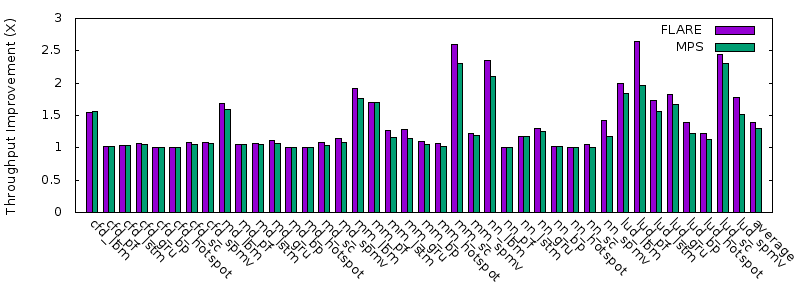
\includegraphics[width=\textwidth, height=2.5cm]{figures/thrpt_res_15.png}
        %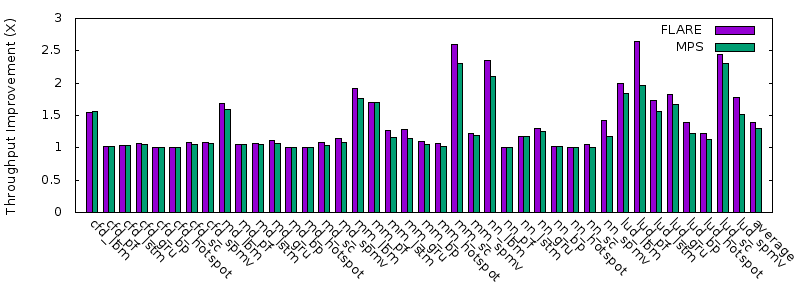
\includegraphics[width=\textwidth]{figures/thrpt_res_15.png}
    %    %\vspace{-0.5cm}
        \caption{Throughput Improvement at 1.5X QoS}
        \label{fig:throughput-results}
        \vspace{-0.5cm}
    \end{figure*}\\
    %\vspace{-1.5cm}
    %\begin{figure*}
    %    \centering
    %    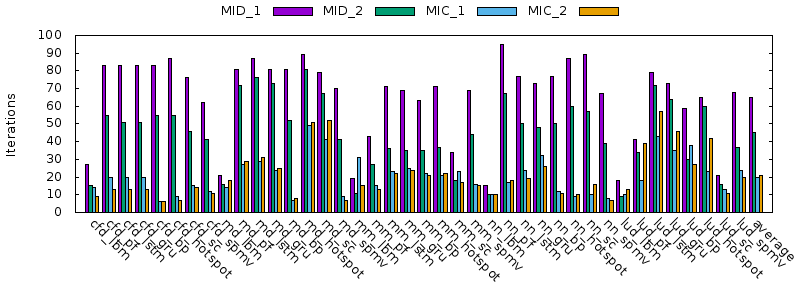
\includegraphics[width=\textwidth, height=2.5cm]{figures/oh_res_12.png}
    %    %\vspace{-0.5cm}
    %    \caption{Online searching overhead at 1.2X QoS}
    %    \label{fig:overhead-results}
        %\vspace{-1cm}
    %\end{figure*}
	%\begin{figure*}
	%	\centering
	%	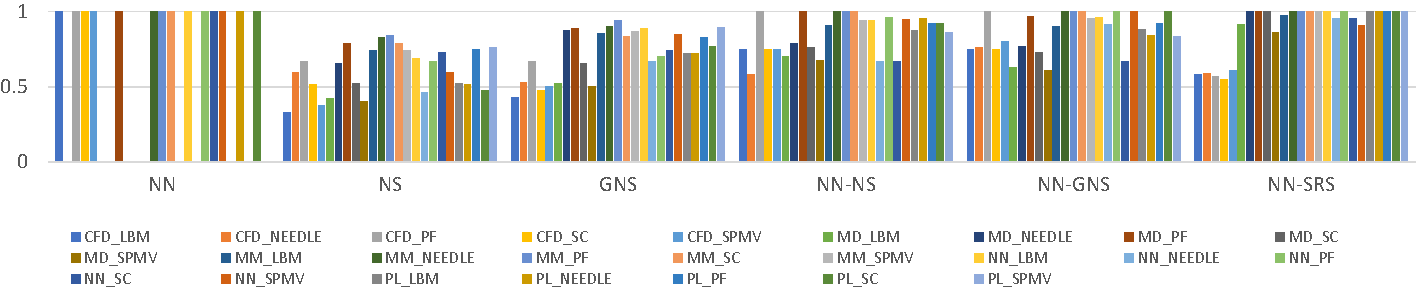
\includegraphics[width=\textwidth]{figures/config_qos_hits_cropped.pdf}
	%	\caption{QoS satisfaction rates of the explored configurations during search.}
	%	\label{fig:config-qos-rate}
	%	%\vspace{-0.5cm}
	%\end{figure*}
%Although the final chosen configuration satisfies QoS as long as dynamic searching is adopted,
%the QoS may be violated during the search process. 
%We observe that the hybrid approaches satisfy QoS more frequently than
%the dynamic only approaches because NN chooses a ``good'' initial configuration and avoids the exploration of configurations
%far from the optimal one.
%\nsout{Figure~\ref{fig:config-qos-rate} shows the fraction of
%iterations which satisfy QoS, where the remainder violate QoS due to choosing detrimental configurations.
%\vspace{1cm}
%\textbf{NN} only explores one configuration, so it either satisfies the QoS %(the bar is of height 1) 
%or misses it. %target, 
%We find that 19 out of 40 co-runs violate QoS in \textbf{NN}. %,
%which makes the NN-only approach unacceptable. %Although the final chosen configuration satisfies QoS as long as dynamic searching is adopted,
%the QoS may be violated during the search process. We observe that the hybrid approaches satisfy QoS more frequently than
%the dynamic only approaches because NN chooses a ``good'' initial configuration and avoids the exploration of configurations
%far from the optimal one.  \\

    \begin{figure*}
    \vspace{-0.5cm}
        \centering
        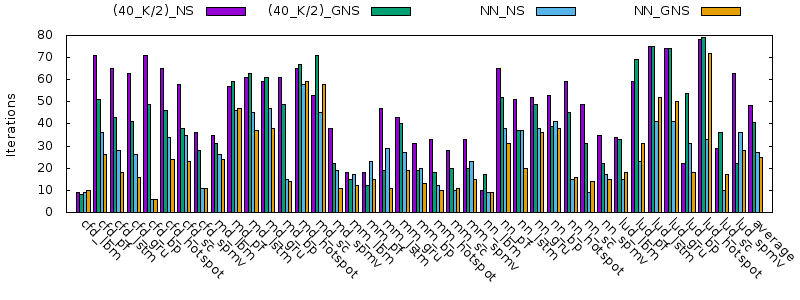
\includegraphics[width=\textwidth, height=2.5cm]{figures/oh_res_15.png}
        %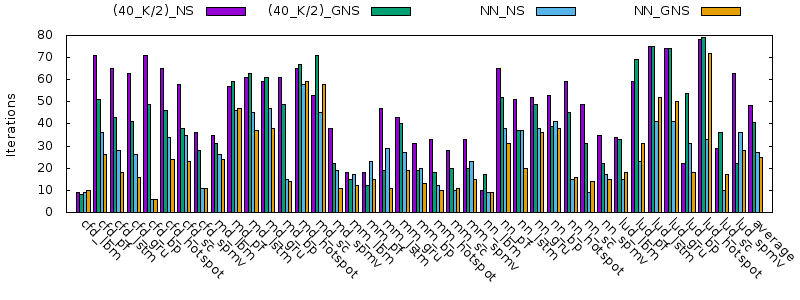
\includegraphics[width=\textwidth]{figures/oh_res_15.png}
        %\vspace{-0.5cm}
        \caption{Online searching overhead at 1.5X QoS}
        \label{fig:overhead-results}
        \vspace{-0.6cm}
    \end{figure*}\\
	%\begin{figure*}%3 out 40 case.\\%and 1 out 40 cases for QoS as 1.2 and 1.5 times of solo-run.
 %The results demonstrate the benefits from spatial
%co-runs enabled by FLARE, which is a key distinction from previous systems.\\
%\subsection{Micro-benchmark Based Performance Degradation Prediction}
\textbf{\textit{Micro-benchmark Prediction Error:}}
%\vspace{-0.5cm}
Fig.~\ref{fig:error} shows the relative error of the performance degradation of LC applications and the relative error of overall throughput predicted
by the \textbf{NN} method for each of the BE and LC kernels. % when QoS is set as 1.2X LC solo-run time. 
%TT and LC in the figure stands for the predictions of overall throughput and latency. %Given the performance degradation of an application as $D$ 
%and the predicted performance degradation due to a co-run as $D'$, 
The relative error is
defined as $|D'-D|/max(D, D')$. The results demonstrate the inefficiency of %the challenge of relying on
model-based approaches to predict performance degradation. For NN\_PF, the prediction
error for %overall 
throughput %of MD\_PF 
and the LC degradation is 
89\% and 92\%, respectively. 
 They are  39\% and 18\% for MM\_PF. The reason is that the applications have
dramatically different properties, such as memory access pattern and branch divergence,
which are difficult to accurately characterize using microbenchmarks. Fortunately, the 
microbenchmarks still capture important features relevant to co-running for a number of
benchmarks. For instance, the prediction errors are as low as 3\% (overall throughput) and 1\% (LC latency) for
CFD\_BP. % co-run. 
On average, the \textbf{NN} method produces 37\% prediction error for the %overall 
throughput and 51\% error for LC latency. % of LC applications. 
Therefore, it is reasonable to use the 
\textbf{NN} method to choose an initial configuration for online search. %Since NN approach does a better job than linear regression
%we do not present detailed data for the linear regression method, which produces much larger (about $2X$ to $5X$) 
%error than nearest neighbor method. 
The NN\_PF pair is an exception in all the pairs. %PF does not like to pair with NN. %If PF co-runs with NN, its performance get hurt significantly. 
No matter how the resources are allocated to PF, the degradation is 15X,
which is why the prediction errors %
%and throughput 
are so large.\\%\vspace{-0.3cm}
    %\begin{figure*}
    %    \centering
    %    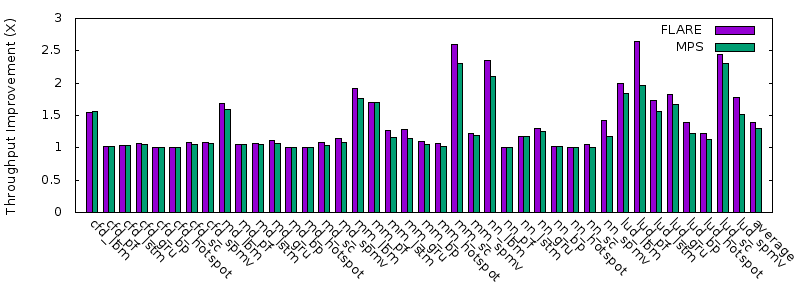
\includegraphics[width=\textwidth,height=2.5cm]{figures/thrpt_res_15.png}
        %\vspace{-0.5cm}
    %    \caption{Throughput Improvement at 1.5X QoS}
    %    \label{fig:throughput-results-1}
        %\vspace{-1cm}
    %\end{figure*}
    %\vspace{-1cm}
    %\begin{figure*}
    %    \centering
    %    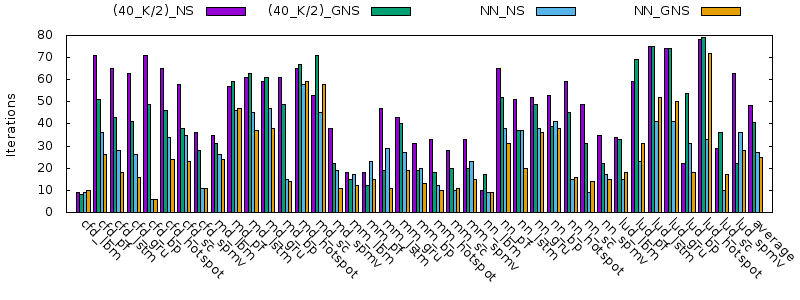
\includegraphics[width=\textwidth, height=2.5cm]{figures/oh_res_15.png}
        %\vspace{-0.5cm}
    %    \caption{Online Searching Overhead at 1.5X QoS}
    %    \label{fig:overhead-results-1}
        %\vspace{-1cm}
    %\end{figure*}
%\subsection{Results on Real Applications}
\textbf{\textit{Real Applications:}}
%\begin{figure}
%		\centering
%		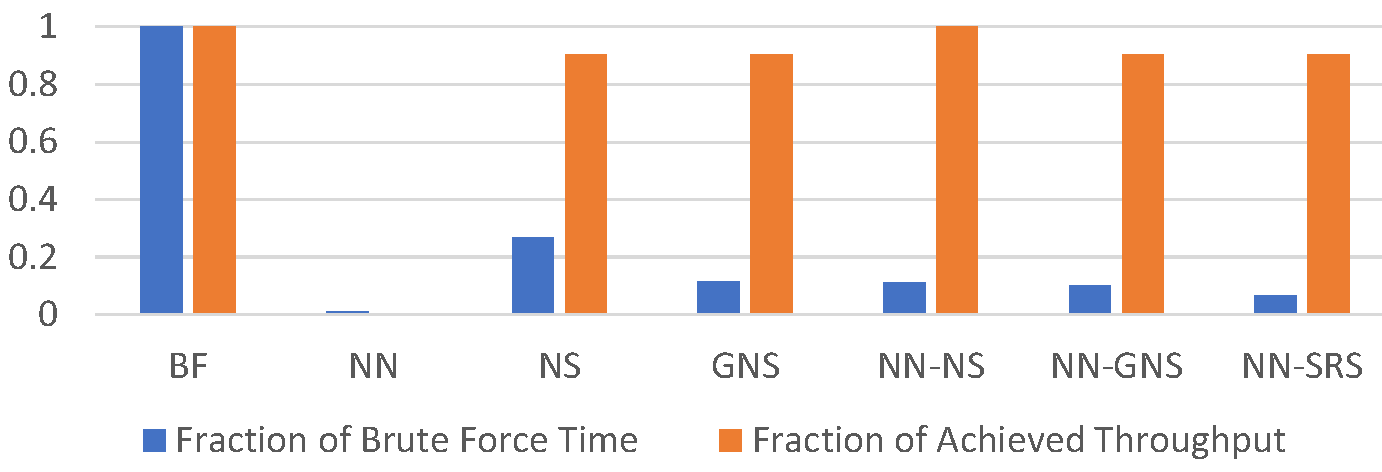
\includegraphics[width=8cm]{figures/real_config_results_cropped.pdf}
%		%\vspace{-0.5cm}
%		\caption{Achieved throughput and runtime overhead when running real applications.}
%		\label{fig:real-config-results}
%	\end{figure}
	%\begin{figure}
	%	\centering
	%	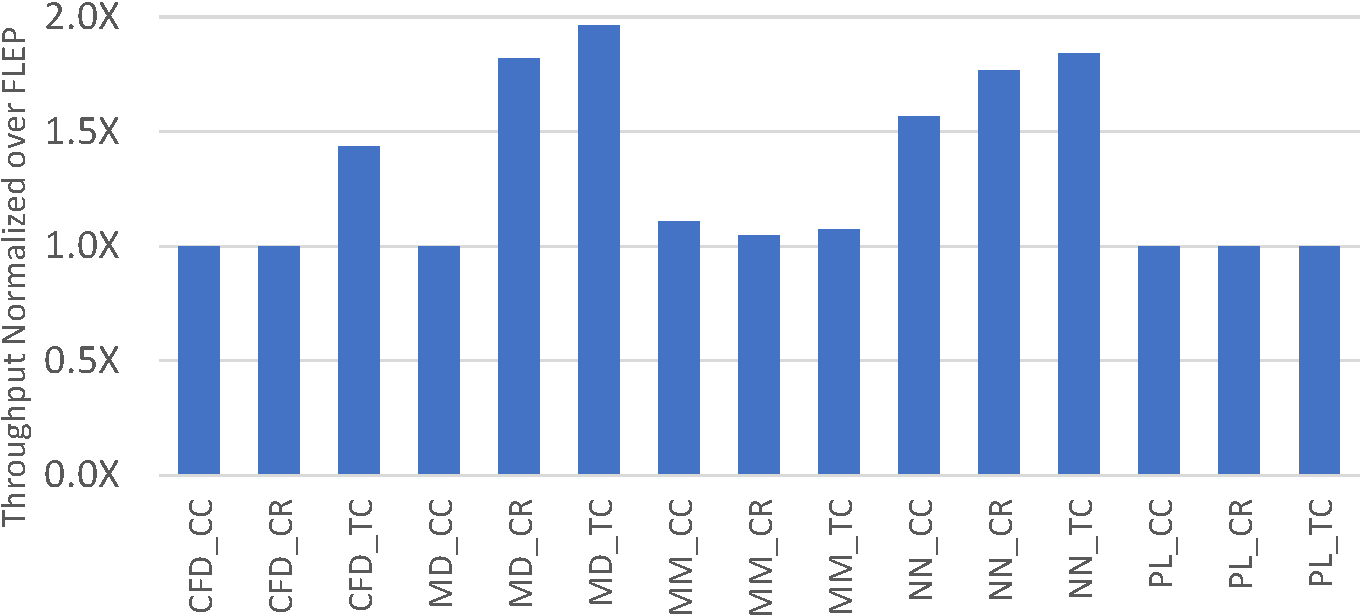
\includegraphics[width=8cm]{figures/real_advantage_cropped.pdf}
	%	\caption{Improvement on hardware utilization when running real applications.}
	%	%\vspace{-0.5cm}
	%	\label{fig:real-advantage}
	%\end{figure}
%We run the two real-world applications (LSTM and GRU) as LC applications paired with 5 benchmarks as BE applications in FLARE.
Fig.~\ref{fig:throughput-results} %and \ref{fig:throughput-results-1} 
show the average throughput improvement across all the co-run pairs including real-world applications for different approaches.
%choosing the co-run configuration that satisfies QoS target.%two objectives of interest at two different QoS target. 
Fig. \ref{fig:overhead-results} %and \ref{fig:overhead-results-1} 
illustrates overheads to
find resource configurations for real-world applications. The pair enclosed in parentheses indicates the initial configuration where $MK$ is the number of maximum thread blocks an SM can host. Similar to the results on benchmarks, \textbf{NN} incurs minimum overhead. \textbf{NN} and \textbf{GNS} %the pure
%dynamic approaches 
need a long search process evidenced by the substantial runtime overhead.
\textbf{NN}, unfortunately, cannot find any configuration that satisfy QoS and hence results from the \textbf{NN} method are not included in these figures.
Dynamic searching algorithms %NN\_NS 
achieve the optimal overall throughput in all the 10 cases. % for two QoS targets.
The average throughput improvement of LSTM and GRU for 5 different pairs is 26\% and 32\%, respectively. %, at 1.2X QoS and they are 46\% and 28\%, respectively for 1.5X QoS.
%The tables \ref{tab:ro-12} and \ref{tab:ro-15} show the overheads of LSTM and GRU pairs at two QoS targets for 4 different approaches. 
The microbenchmark-based methods outperform \textbf{NN} and \textbf{GNS}. %the searches starting at initial guess at (40, 4). 
The overheads with microbenchmark guidance are about 60\% of \textbf{NN} and \textbf{GNS}.% at 1.2 QoS. 
%The former spend about $2/3$ of the time of guess (40, 4) for 1.5 QoS on dynamical searches for the best configuration. 
%\begin{table}
%\begin{minipage}{0.5\linewidth}
    %\centering
%    \begin{tabularx}{\linewidth}{c c c c c}
%    \hline \hline
%         Pair & NN\_NS\_MID & NN\_GNS\_MID & NN\_NS\_MIC & NN\_GNS_MIC \\ \hline
%         LSTM &  79 & 57 & 24 & 28 \\
%         GRU  &  76 & 54 & 27 & 23 \\ 
%         \hline
%    \end{tabularx}
%    \caption{Real-world Pairs Overhead at 1.2X QoS}
%    \label{tab:ro-12}

%\end{minipage}
%\hfill
%\begin{minipage}{0.5\linewidth}
    %\centering
%    \begin{tabularx}{\linewidth}{c c c c c}
%    \hline \hline
%         Pair & NN\_NS\_MID & NN\_GNS\_MID & NN\_NS\_MIC & NN\_GNS_MIC \\ \hline
%         LSTM &  59 & 47 & 44 & 33 \\
%         GRU  &  58 & 51 & 43 & 34 \\ 
%         \hline
%    \end{tabularx}
%    \caption{Real-world Pairs Overhead at 1.5X QoS}
%    \label{tab:ro-15}
%\end{minipage}
%\end{table}
%The overheads of LSTM pairs for 4 approaches (NN\_MID\_1,NN\_MID\_2, NN\_MIC\_1 and NN\_MIC\_2) are 79, 57, 24, and 28 at 1.2X QoS. They are 76, 54, 27, and 23 for GRU pairs.
%At 1.5X QoS, average LSTM and GRU overheads are 

%\vspace{-0.5cm}
\section{Related Work}
\vspace{-0.2cm}
%GPU workload characterization has been studied for over a decade. Reference \cite{Liworkloads} proposed a set of characterizing a workload
%to evaluate the performance of a GPU microarchitecture. However, our concern is the impact of resource contentions 
%on the performance of multiple applications. In FLARE, the performance affected by a specific GPU architecture is simulated by the data 
%of those carefully designed microbenchmarks run offline.
%Performance prediction and resource partitioning for co-located applications on CPU 
%platforms have attracted significant attention. Bubble-Up~\cite{Mars:MICRO2011},
%Octopus-Man~\cite{Petrucci:HPCA2015}, and SMiTe~\cite{Zhang:2014} use profiling data of 
%the target applications to characterize performance degradation on real CPU systems, 
%but the LC applications may be submitted by data center users and hence not available 
%for detailed profiling and characterization. In comparison, we do not assume the
%availability of the LC applications and purely rely on micro benchmarks and online 
%configuration search to guarantee QoS. Multiple systems use online profiling and
%adaptive resource partitioning to provide flexibility~\cite{Zhu+:ASPLOS16,Lo:2015}, 
%but unlike FLARE they do not leverage micro benchmarks to reduce search overhead.
%Moreover, researchers have proposed cache partitioning approaches to guaranteeing QoS 
%of LC applications~\cite{Kasture:ASPLOS14,Lin:HPCA08,Ye:PACT14,Sayed:HPCA18} on CPUs.
%A linear model is assumed in SMiTe. However, our experiments have shown that linear model doesn't work well for GPU.
Researchers have proposed architectural extensions to allow %\nsout{efficient application}{}
applications to co-run efficiently
on the same GPU, with emphasis on cache sharing and bypassing~\cite{Liang:ICCAD17},
fine-grained sharing~\cite{Wang:ISCA2017},
preemption~\cite{Park+:ASPLOS15,Tanasic+:ISCA14}, dynamic resource management~\cite{Park:ASPLOS17}, 
and spatial multi-tasking~\cite{Adriaens+:HPCA12,slate2019}. The work \cite{Wang:ISCA2017} deals with spatial sharing through an enhanced scheduler (both thread block and warp level) to 
guarantee QoS. They use a quota to represent the QoS constraint. They assume that thread blocks are uniform in cost and the quota needs to reach zero at each epoch to satisfy QoS. To further improve 
the performance, they implement dynamic resource allocation by monitoring idle warps during each epoch. %The idle warp counter and enhanced scheduler
%are rarely available to a programmer. }
On the one hand, those techniques remain to be
carefully evaluated for implementation in real GPUs. On the other hand, those studies do
not systematically address reducing search overhead to find the best strategy for GPU sharing. 
Studies~\cite{Liang:TPDS15} have demonstrated 
that multi-tasking on GPUs can better utilize the hardware resource, 
but none of them predict performance degradation due to the co-running. 
Software systems, such as FLEP~\cite{Wu:ASPLOS2017} and EffiSha~\cite{Chen:PPoPP2017},
focus on lightweight preemption support but do not particularly study QoS enforcement.
Baymax~\cite{Chen+:ASPLOS16} and Prophet~\cite{Chen:ASPLOS2017} predict GPU workload
performance and use task re-ordering to handle QoS. 
Their approach to coordinate data transfers can be directly incorporated in 
FLARE to form a more general solution. Since they assume the GPUs are non-preemptable, % co-processors, 
they may use FLARE's methodology to further improve GPU utilization.\\
Another line of interesting work is practical GPU sharing in virtual environments, 
for which Hong et al. provide a comprehensive survey~\cite{Hong:ACSU}. 
We briefly discuss several closely related studies. FairGV~\cite{Hong:TPDS17} 
achieves system-wide weighted fair sharing among GPU applications through 
collaborative scheduling and an accurate accounting mechanism. 
Gloop~\cite{Suzuki:SOCC17} proposes a new programming model to generate scheduling points in GPU kernels, 
which enables flexible suspending/resuming execution of GPU applications. 
Tian et al. propose a software system to virtualize Intel on-chip GPUs for graphics workloads~\cite{Tian+:ATC14}. 
None of these approaches have addressed fine-grained sharing or QoS of user-facing applications. 
To share the GPU memory %between applications, 
GPUvm~\cite{Suzuki+:ATC14} partitions 
the GPU memory into regions and assign the regions to virtual machines. 
GPUswap~\cite{Kehne+:VEE15} automatically coordinates GPU memory usage between applications 
even if the aggregate workload does not fit in GPU physical memory. 
%Although GPU virtualization solve the co-run to a certain extent, 
%the purpose of the virtualization is to separate GPU environment so that one application would not experience the existence of other applications. 
%Though FLARE is focused on the sharing of computational resources, 
%there is a potential to integrate these approaches in FLARE into hypervisor of GPU virtualization to provide a more comprehensive system. 


\section{Conclusion}
\vspace{-.2cm}
GPU sharing is a promising approach to improving hardware utilization, but resource
contention may degrade the performance of the co-running latency-critical applications to
violate QoS. In this paper, we demonstrated the complexities of partitioning GPU resources
to enforce QoS and maximize throughput. To address the challenges, we proposed a software
system named FLARE to enable and configure spatial GPU sharing between latency-critical
and best-effort applications through kernel transformation, micro-benchmark guided
partitioning and online configuration search. The experiment results showed 39\% improvement on the overall throughput on 11 benchmarks and 2 real-world
applications over existing systems. In the future, we plan to extend FLARE to address scenarios in which multiple latency-critical applications share the same GPU.%\vspace{-0.6cm}

%\bibliographystyle{ACM-Reference-Format}
\bibliographystyle{plain}
\bibliography{all}

\end{document}

